% inmersionEnPython.tex
% This work is licensed under the Creative Commons Attribution-Noncommercial-Share Alike 3.0 New Zealand License.
% To view a copy of this license, visit http://creativecommons.org/licenses/by-nc-sa/3.0/nz
% or send a letter to Creative Commons, 171 Second Street, Suite 300, San Francisco, California, 94105, USA.

\documentclass[12pt,leqno,a4paper,spanish]{book}
\usepackage[dvips]{graphicx}
\usepackage[dvipsnames,usenames]{color}
\usepackage{makeidx}
\usepackage[absolute]{textpos}
\usepackage{wrapfig}
\usepackage{eso-pic}
\usepackage[utf8]{inputenc}
\usepackage{mathabx}
\usepackage{babel}
\usepackage{listings}
\usepackage[colorlinks,unicode]{hyperref}
\hypersetup{
    pdfauthor={Jos\'{e} Miguel Gonz\'{a}lez Aguilera},
    pdftitle={Inmersi\'{o}n en Python 3},
    pdfsubject={Programaci\'{o}n en Python 3},
    pdfkeywords={python,python 3,programaci\'{o}n}
}
\parindent 1cm
\parskip 0.2cm
\topmargin 0.2cm
\oddsidemargin 1cm
\evensidemargin 0.5cm
\textwidth 15cm
\textheight 21cm

\graphicspath{{./imagen/}}

\hyphenation{Python}

\newcommand{\cajaTexto}[1]
{\begin{wrapfigure}{r}{.4\linewidth}\fbox{\colorbox{gray}{\parbox{.9\linewidth} {#1}}}\end{wrapfigure}}

\newenvironment{citaCap}
{\begin{flushright}\begin{itshape}}
{\end{itshape}\end{flushright}}

\newenvironment{listing}
{\begin{list}{}{\setlength{\leftmargin}{1em}}\item\footnotesize\samepage}
{\end{list}}

\newcommand{\ac}[1]{\textrm{\'{#1}}}
\newcommand{\til}[1]{\textrm{\~{#1}}}

\newcommand{\codigo}[1]{\textsf{#1}}

\newcommand{\difl}{$\blackdiamond\diamond\diamond\diamond\diamond$}

\newcommand{\difll}{$\blackdiamond\blackdiamond\diamond\diamond\diamond$}

\newcommand{\diflll}{$\blackdiamond\blackdiamond\blackdiamond\diamond\diamond$}

\newcommand{\difllll}{$\blackdiamond\blackdiamond\blackdiamond\blackdiamond\diamond$}

\newcommand{\diflllll}{$\blackdiamond\blackdiamond\blackdiamond\blackdiamond\blackdiamond$}

\setcounter {chapter}{-2}

\newcommand{\code}{\textcolor{OliveGreen}\bfseries}

\title{Inmersión en Python 3}
\author{Mark Pilgrim}

\makeindex

\definecolor{gray}{rgb}{0.98,0.98,0.98}
\definecolor{black}{rgb}{0,0,0}

\begin{document}
\widowpenalty=10000
\clubpenalty=10000
\raggedbottom
\lstset{language=Python,showstringspaces=false,numbers=left,
        numberstyle=\footnotesize,backgroundcolor=\color{gray},
        rulesep=1pt, rulesepcolor=\color{black},frame=leftline,
        basicstyle=\footnotesize, mathescape=true}
\pagestyle{headings}
\pagenumbering{arabic}

% ch1.tex
% This work is licensed under the Creative Commons Attribution-Noncommercial-Share Alike 3.0 New Zealand License.
% To view a copy of this license, visit http://creativecommons.org/licenses/by-nc-sa/3.0/nz
% or send a letter to Creative Commons, 171 Second Street, Suite 300, San Francisco, California, 94105, USA.

\chapter{Novedades de ``Inmersión en Python 3''}\label{ch:novedades}

\begin{citaCap}
``¿No es de aquí de donde venimos?''\\
---Pink Floyd, The Wall
\end{citaCap}

\section{Alias ``Bajo el nivel del mar''}

Posiblemente hayas leído el libro original \emph{Dive into Python} y puede que hasta lo hayas comprado. (Si es el caso: ¡gracias!) Ya conoces bastante el lenguaje Python. Estás preparado para dar el salto a Python 3. \ldots Si lo dicho es cierto, sigue leyendo. (Si no es así, tal vez sea mejor que comiences desde el principio en el capítulo~\ref{ch:instalandopython}).

Python 3 viene con un script denominado \codigo{2to3}. Aprende a usarlo y a quererlo. El apéndice~\ref{ap:convirtiendocodigo} es una referencia sobre las cosas que la herramienta \codigo{2to3} puede realizar automáticamente. Puesto que muchas cosas son cambios de sintaxis, una buena forma de comenzar es aprender estas diferencias. Por ejemplo: \codigo{print} ahora es una función, `x` no funciona, etc.

El caso de estudio del capítulo~\ref{ch:casodeestudio} documenta mi esfuerzo (¡al fin cumplido con éxito!) de convertir una librería real de Python 2 a Python 3. Puede servirte o no. Es un ejemplo complejo de entender puesto que en primer lugar tienes que comprender algo el funcionamiento de la librería, de forma que puedas entender lo que deja de funcionar y como lo arreglé.  Mucho de lo que se rompió al pasar a la versión 3 de Python fue por causa de las cadenas.  Por cierto, hablando de cadenas\ldots

Cadenas. ¡Uff!. Por dónde podría empezar. Python 2 tenía ``cadenas'' y ``cadenas unicode''. Python 3 tiene ``bytes'' y ``cadenas''. Lo que significa que todas las cadenas ahora son unicode, y si quieres trabajar con un puñado de bytes tienes que usar el tipo \textbf{bold} bytes.

Python 3 nunca convertirá implícitamente entre cadenas y bytes, por lo que si no estas seguro de lo que contiene una variable en un momento dado, el código seguro que fallará en algún momento. Lee el capítulo~\ref{ch:cadenas} sobre cadenas para conocer los detalles.

La división entre ``bytes'' y ``cadenas'' surgirá en diversas partes del libro:

\begin{enumerate}
\item En el capítulo~\ref{ch:ficheros} dedicado a los ficheros, aprenderás la diferencia entre leer ficheros en modo \emph{binario} o en modo \emph{texto}. La lectura (y escritura) de ficheros en modo \emph{texto} requiere que se utilice el parámetro \codigo{encoding}. Existen métodos que cuentan los caracteres de un fichero y métodos que cuentan bytes. Si el código asume que un carácter es igual a un byte, no funcionará cuando el fichero contenga caracteres multibyte\footnote{En unicode muchos caracteres se representan utilizando más de un byte}.

\item En el capítulo~\ref{ch:httpserviciosweb} dedicado a los servicios web n http, se muestra el módulo \codigo{httplib2} que lee cabeceras y datos de \codigo{HTTP}. Las cabeceras se obtienen como cadenas, pero el contenido del cuerpo se obtiene como bytes.

\item En el capítulo~\ref{ch:serializandoobjetos} aprenderás el motivo por el que el módulo \codigo{pickle} de Python 3 define un formato de datos nuevo que es incompatible con Python 2 (Pista: Se debe a los bytes y cadenas). También afecta al módulo \codigo{JSON}, que no es capaz de manejar el tipo \codigo{bytes}. Te enseñaré como salvar este escollo.

\item En el capítulo~\ref{ch:casodeestudio} sobre la conversión de la librería \codigo{chardet} a Python 3 se verá que la mayor parte de los problemas de conversión provienen de los bytes y cadenas.
\end{enumerate}

Incluso aunque no tengas interés en Unicode, ¡que tendrás!, querrás leer sobre el formateo de cadenas en Python 3 en el capítulo~\ref{ch:formateodecadenas}, que es completamente diferente a Python 2.

Los iteradores están en todas partes en Python 3, y ahora los entiendo mucho mejor que hace cinco años cuando escribí ``Inmersión en Python''. Debes comprenderlos tú también, puesto que muchas funciones que anteriormente retornaban listas ahora, en Python 3, devuelven iteradores. Como mínimo, deberías leer la segunda parte del capítulo~\ref{ch:iteradores} dedicado a los iteradores y la segunda parte del capítulo~\ref{ch:iteradoresavanzados} sobre el uso avanzado de los iteradores.

Por petición popular, he añadido el apéndice~\ref{ap:nombresdemetodosespeciales} sobre nombres de método especiales que guarda cierta similitud con el apartado similar de la \href{http://www.python.org/doc/3.1/reference/datamodel.html#special-method-names}{documentación oficial de Python 3} pero con cierta ironía.

Cuando estaba escribiendo ``Inmersión en Python'' todas las librerías de XML disponibles eran bastante malas. Entonces Fedrik Lundh escribió \textbf{bold} \href{http://effbot.org/zone/element-index.htm}{ElementTree}, que es todo lo contrario a lo existente anteriormente. Los dioses de Python, actuando inteligentemente, \href{http://docs.python.org/3.1/library/xml.etree.elementtree.html}{incorporaron ElementTree a la librería estándar}. Ahora esta librería es el fundamento del capítulo~\ref{ch:xml} sobre XML. Los viejos métodos para recorrer XML están aún disponibles, pero deberías evitarlos, ¡apestan!

Algo que es también nuevo ---no en el lenguaje, pero sí en la comunidad--- es la creación de repositorios de código como \href{http://pypi.python.org/}{el índice de paquetes de python (PyPI)}. Python dispone de utilidades para empaquetar el código en formatos estándares y distribuirlos en PyPI. Lee el capítulo~\ref{ch:empaquetandolibrerias} sobre  cómo empaquetar librerías en Python.
\newpage

% ch0.tex
% This work is licensed under the Creative Commons Attribution-Noncommercial-Share Alike 3.0 New Zealand License.
% To view a copy of this license, visit http://creativecommons.org/licenses/by-nc-sa/3.0/nz
% or send a letter to Creative Commons, 171 Second Street, Suite 300, San Francisco, California, 94105, USA.

\chapter{Instalación de Python}\label{ch:instalacion}

\noindent
Nivel de dificultad:\difl

\begin{citaCap}
``Tempora mutantur nos et mutamur in illis''\\
(Los tiempos cambian, y nosotros cambiamos con ellos)\\
---antiguo proverbio romano
\end{citaCap}

\section{Inmersión}

Bienvenido a Python 3. ¡Vamos a mojarnos! En este capítulo, vas a instalar la versión de Python adecuada para ti.

\section{¿Cuál es la versión adecuada para ti?}

Lo primero que necesitas hacer es instalar Python 3.

Si estás utilizando una sesión en un servidor remoto (posiblemente a través de Internet), el administrador del servidor puede que ya lo haya instalado por ti. Si estás utilizando Linux\footnote{Nota del Traductor: El nombre correcto del sistema operativo Linux es GNU/Linux, no obstante, por comodidad, en este libro se utilizará únicamente Linux para mayor comodidad} en casa, puede que también lo tengas ya instalado, aunque actualmente\footnote{año 2009} la mayor parte de las distribuciones de Linux vienen con Python 2 instalado (como verás en este capítulo, puedes tener simultáneamente más de una versión de Python en tu ordenador sin problemas). En los Mac OS X se incluye una versión de línea de comando de Python 2, pero no Python 3. Microsoft Windows no trae ninguna versión de Python. Pero ¡no te preocupes! siempre puedes instalarlo tú mismo, tengas el sistema operativo que tengas.

La forma más sencilla para comprobar si tienes instalado Python 3 en tu sistema Linux o Mac OS X es abrir un terminal de línea de comandos. Para ello debes hacer lo siguiente:

\begin{itemize}
\item Si estás en Linux, busca en el menú de \codigo{Aplicaciones} un programa denominado \codigo{terminal} (puede estar en un submenú, posiblemente \codigo{Accesorios} o \codigo{Sistema}).
\item Si estás en Mac OS X, existe una aplicación que se llama \codigo{Terminal.app} en la carpeta \codigo{/Aplicaciones/Utilidades/}.
\end{itemize}

Una vez te encuentres en la línea de comando\footnote{También conocido como el ``prompt''}, teclea \codigo{python3} (en minúsculas y sin espacios) y observa lo que sucede. En mi sistema Linux, Python 3 ya está instalado, por lo que el resultado de ejecutar este comando hace que el terminal entre en la \emph{consola\footnote{En inglés ``shell''} interactiva de Python}.
\begin{listing}
\begin{verbatim}
jmgaguilera@acerNetbook-jmga:~$ python3
Python 3.0.1+ (r301:69556, Apr 15 2009, 15:59:22) 
[GCC 4.3.3] on linux2
Type "help", "copyright", "credits" or "license" for more information.
>>> 
\end{verbatim}
\end{listing}

(Para salir de la consola interactiva de Python escribe \codigo{exit()} y pulsa la tecla \codigo{INTRO}.)

Al ejecutar esta misma sentencia \codigo{python3} en un ordenador Linux que no tenga instalado Python 3 el mensaje que se obtendrá será parecido al siguiente:

\begin{listing}
\begin{verbatim}
jmgaguilera@acerNetbook-jmga:~$ python3
bash: python3: orden no encontrada
jmgaguilera@acerNetbook-jmga:~$ python3
\end{verbatim}
\end{listing}

Bueno, volviendo ahora a la pregunta sobre cuál es la versión de Python 3 apropiada para ti, queda claro que es aquella que se ejecute en el ordenador que tengas.

Para conocer cómo instalar Python 3, continúa leyendo en el apartado que corresponda a tu sistema operativo.

\section{Instalación en Microsoft Windows}

Windows se ejecuta actualmente en dos plataformas diferentes: 32 y 64 bits. Asimismo, existen diferentes \emph{versiones} de Windows ---XP, Vista, Windows 7--- y Python 3 funciona en todas ellas. Es más importante, con vistas a la instalación, la distinción que existe entre los dos tipos de arquitecturas. Si no sabes de qué tipo es la arquitectura de tu ordenador, lo más probable es que sea de 32 bits.

Visita \href{http://python.org/download/}{python.org/download/} para descargar la aplicación de instalación de Python 3 que sea correcta para para la arquitectura de tu ordenador. Las posibilidades serán parecidas a:

\begin{itemize}
\item \textbf{Python 3.*.* x86 Windows installer} (Windows binary --- does not include sources)
\item \textbf{Python 3.*.* AMD64 Windows installer} (Windows AMD64 binary --- does not include sources)
\end{itemize}

La descarga exacta varía en función de las actualizaciones. Por eso he puesto asteriscos en lugar del número de versión. Deberías instalar siempre la última versión disponible de Python 3.x a menos que tengas alguna razón importante para no hacerlo.

\begin{figure}[!h]
  \begin{center}
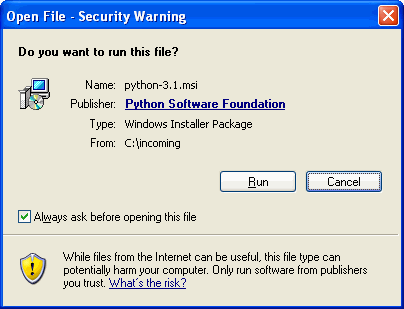
\includegraphics[width=0.5\textwidth]{winInstalacion1.png}
\caption{Advertencia al inicio}\label{fig01}
  \end{center}
\end{figure}

Cuando la descarga finalize, pulsa (doble click) sobre el fichero \codigo{.msi} que has descargado. Windows mostrará una alerta de seguridad (figura~\ref{fig01}) para avisarte de que estás intentando ejecutar un fichero que instalará cosas en tu ordenador. El fichero instalador de Python está firmado electrónicamente por la \href{http://www.python.org/psf/}{\emph{Python Software Foundation}}, que es la organización sin ánimo de lucro que supervisa el desarrollo de Python. ¡No aceptes imitaciones!

Pulsa el botón \codigo{Run} o \codigo{Ejecutar}\footnote{dependerá del idioma en el que se encuentre tu sistema operativo} para que se inicie la ejecución del programa instalador de Python.

\begin{figure}[!h]
 \begin{center}
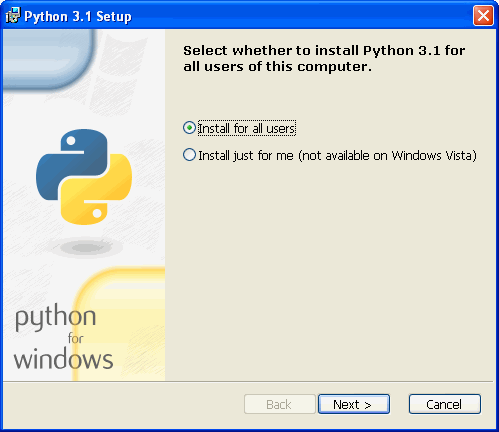
\includegraphics[width=0.5\textwidth]{winInstalacion2.png}
\caption{Tipo de instalación}\label{fig02}
  \end{center}
\end{figure}

Lo primero que pide el programa instalador (figura~\ref{fig02}) es que le indiques si quieres instalar Python 3 para todos los usuarios del ordenadores o únicamente para ti. Por defecto aparece seleccionada la opción ``Instalar para todos los usuarios'', que es la mejor opción, a no ser que tengas una buena razón para no hacerlo\footnote{Una posible razón por la podrías querer instalarlo únicamente para tu usuario es que estuvieras instalando Python en el ordenador de la empresa y no tengas permisos de administrador en tu cuenta de usuario. Pero en ese caso, ¿qué haces instalando Python sin permiso del administrador de tu empresa? A mí no me metas en problemas, eso es cosa tuya.}.

Cuando hayas seleccionado la opción deseada, pulsa el botón \codigo{Next} o \codigo{Siguiente} para continuar con la instalación.

Lo siguiente que pedirá el instalador (figura~\ref{fig03}) es que le digas el directorio de instalación. El valor por defecto para todas las versiones de Python 3.1.x es \codigo{C:$\backslash$Python31$\backslash$}, que es un valor adecuado para la mayoría de los usuarios. Salvo que tengas una razón específica para cambiarlo, como por ejemplo, que mantengas una unidad separada para la instalación de aplicaciones, puedes usar este directorio para instalar Python.

Para cambiar el directorio de instalación, puedes utilizar las opciones de pantalla o, simplemente, teclear el directorio deseado (con el path completo) en la caja de texto.

\begin{figure}[!h]
  \begin{center}
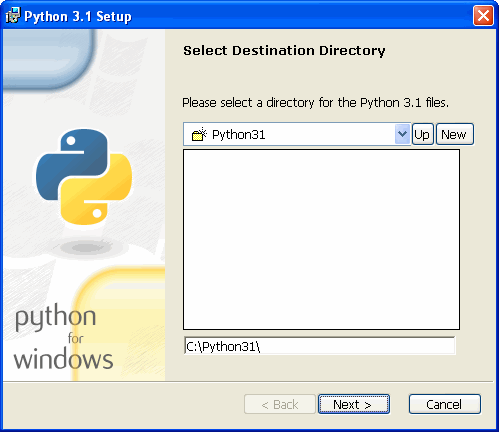
\includegraphics[width=0.5\textwidth]{winInstalacion3.png}
\caption{Directorio de instalación}\label{fig03}
  \end{center}
\end{figure}

Puedes instalar Python en el disco duro en el lugar que desees.

Cuando hayas finalizado, pulsa el botón \codigo{Next} o \codigo{Siguiente} para continuar.

\begin{figure}[!h]
  \begin{center}
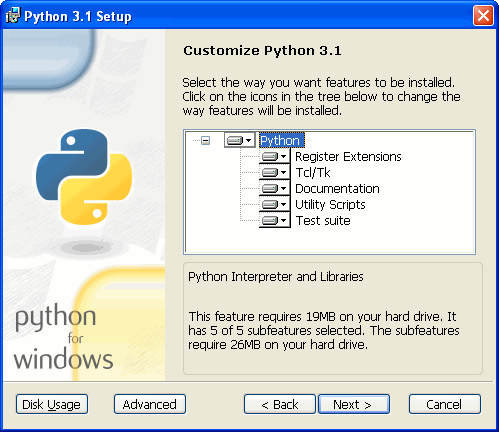
\includegraphics[width=0.5\textwidth]{winInstalacion4.png}
\caption{Selección de elementos a instalar}\label{fig04}
  \end{center}
\end{figure}

La siguiente pantalla (figura~\ref{fig04}) parece más compleja, pero en realidad no lo es. Como pasa con otros muchos instaladores, te ofrece la opción de que selecciones qué cosas concretas quieres instalar. Puedes instalar todos los componentes de Python 3, y si el espacio en disco es justo, puedes excluir ciertos componentes.

\begin{itemize}
\item \textbf{Registrar las extensiones}. Si seleccionas esta opción, el instalador modificará la configuración de Windows para que te permita ejecutar los scripts\footnote{ficheros que contienen sentencias de Python, que normalmente tienen la extensión \codigo{.py}} de Python con solo hacer doble click sobre el fichero. Esta opción no necesita de espacio en disco, por lo que no tiene mucho sentido no marcarla.
\item \textbf{Tcl$\backslash$Tk} es la librería gráfica que utiliza la consola de Python. La usaremos a lo largo de todo el libro, por lo que es muy recomendable que la mantengas entre los componentes a instalar.
\item \textbf{Documentación} instala un fichero de ayuda que contiene gran parte de la información que se encuentra en \href{http://docs.python.org/}{docs.python.org}. Es recomendable instalar esta opción cuando es previsible que no dispongas de conexión permanente a Internet.
\item \textbf{Scripts de utilidades}. Estos scripts incluyen diversas utilidades, entre ellas el script \codigo{2to3.py} sobre el que hablaremos más adelante. Es necesaria si vas a migrar código de Python 2 a Python 3. Si no dispones de código para migrar puedes saltarte esta opción.
\item \textbf{Suite de pruebas.} Es una colección de scripts que se utilizan para probar el buen funcionamiento del intérprete de Python. En este libro no lo vamos a usar, yo no lo he usado jamás en el largo tiempo que llevo programando en Python. Es totalmente opcional su instalación.
\end{itemize}

\begin{figure}[!h]
  \begin{center}
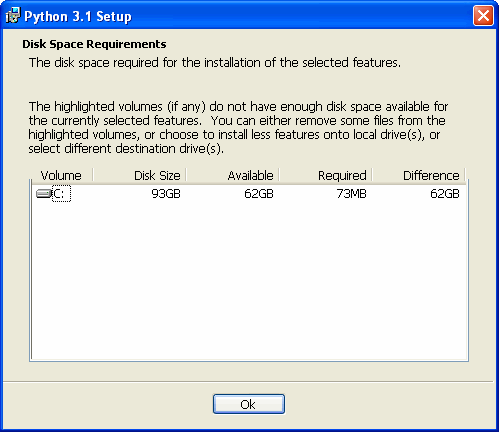
\includegraphics[width=0.5\textwidth]{winInstalacion5.png}
\caption{Espacio libre}\label{fig05}
  \end{center}
\end{figure}

Si no estás seguro de cuando espacio en disco tienes libre, pulsa el botón \codigo{Disk Usage}. El instalador te mostrará las unidades de disco (figura~\ref{fig05}) y el espacio libre disponible en cada una de ellas, así como el espacio que quedará después de la instalación.

Cuando termines la comprobación, pulsa el botón \codigo{OK} para volver a la pantalla anterior.

Si decides excluir alguna opción (figura~\ref{fig06}), selecciona el botón desplegable que aparece a la izquierda del texto de la opción y selecciona \codigo{Entire feature will be unavailable}. Por ejemplo, si excluyes la suite de pruebas ahorrarás 7908 KBytes de espacio en disco.

\begin{figure}[!h]
  \begin{center}
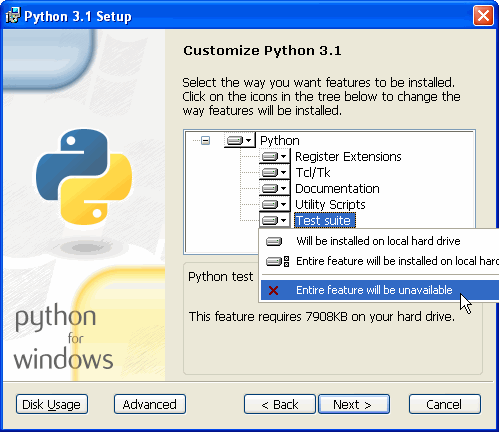
\includegraphics[width=0.5\textwidth]{winInstalacion6.png}
\caption{Excluir una opción}\label{fig06}
  \end{center}
\end{figure}

Pulsa el botón \codigo{Next} para confirmar tu selección de opciones.


\begin{figure}[!h]
  \begin{center}
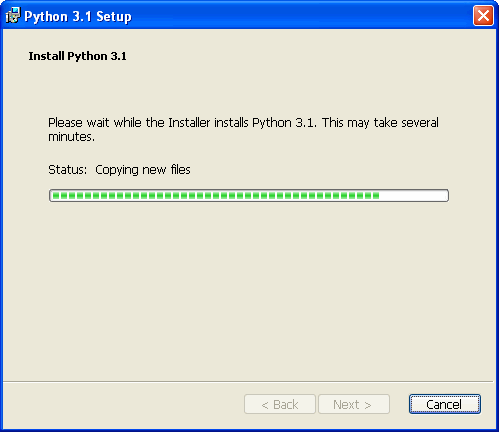
\includegraphics[width=0.5\textwidth]{winInstalacion7.png}
\caption{Instalación}\label{fig07}
  \end{center}
\end{figure}

El instalador copiará todos los ficheros (figura~\ref{fig07} al directorio de destino que hayas seleccionado (Suele ser tan rápido, que tuve que probarlo tres veces antes de conseguir sacar una ``foto'' de la pantalla mostrándolo).
 
\begin{figure}[!h]
  \begin{center}
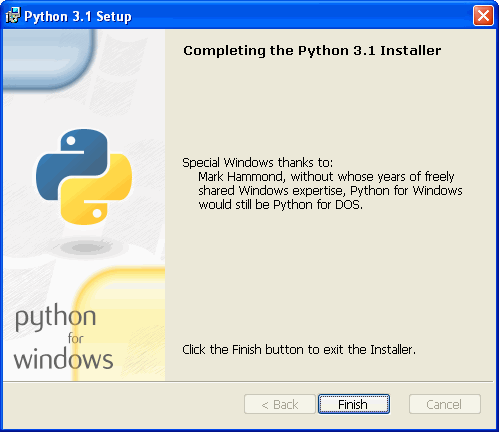
\includegraphics[width=0.5\textwidth]{winInstalacion8.png}
\caption{Instalación completada}\label{fig08}
  \end{center}
\end{figure}

Por último, pulsa el botón \codigo{Finish} para salir del instalador (figura~\ref{fig08}).


\begin{figure}[!h]
  \begin{center}
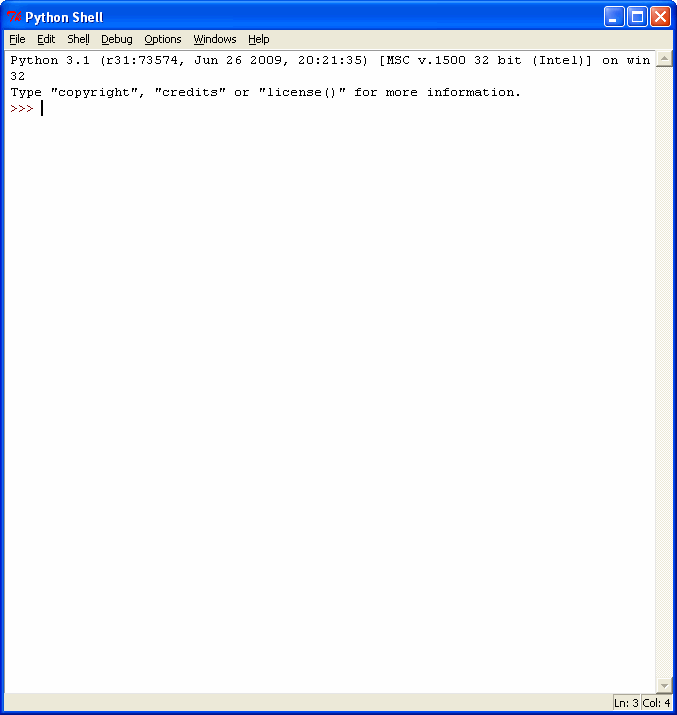
\includegraphics[width=0.5\textwidth]{winInstalacion9.png}
\caption{Instalación completada}\label{fig09}
  \end{center}
\end{figure}

Si ahora buscas en el menú de \codigo{Inicio}, deberías encontrar un nuevo elemento denominado \codigo{Python 3.1}. Dentro de esta nueva opción de menú encontrarás dos programas denominados \codigo{Python} e \codigo{IDLE}. Selecciona uno de estos dos elementos para ejecutar la consola interactiva de Python (figura~\ref{fig09}).

Continúa en el apartado~\ref{sec:shell}

\section{Instalación en un Mac OS X}

Todos los ordenadores Apple Macintosh modernos utilizan procesadores de Intel\footnote{Como la mayoría de ordenadores con Windows} Los Macintosh antiguos utilizaban procesadores Power PC. No es necesario que conozcas esta diferencia puesto que únicamente existe un instalador para todos los tipos de Macs.

Visita \href{http://python.org/download/}{python.org/download/} para descargar la aplicación de instalación de Python 3 para Mac. Debes buscar un enlace cuyo nombre sea algo así como \textbf{Mac Installer Disk Image (3.*.*}. El número de versión puede variar, pero asegúrate de descargar una versión de Python 3 y no de Python 2.


\begin{figure}[!h]
  \begin{center}
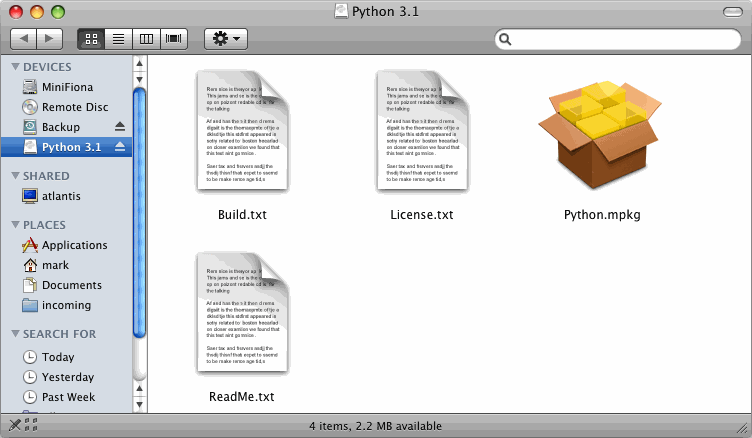
\includegraphics[width=0.5\textwidth]{macInstalacion0.png}
\caption{Finder: contenido de la imagen de disco}\label{figm00}
  \end{center}
\end{figure}

Tu navegador debería montar de forma automática esta imagen de disco y abrir una ventana de \codigo{Finder} para mostrarte el contenido de la imagen. Si no fuese así, deberás buscar la imagen de disco en el directorio de descargas y hacer doble click sobre ella para que se cargue. El nombre de la imagen de disco será algo así como \codigo{python-3-1.dmg}. Una vez tengas visible en pantalla el contenido de la imagen de disco (figura~\ref{figm00}), podrás observar que contiene varios ficheros de texto \codigo{(Build.txt, License.txt, ReadMe.txt)}, y el el fichero del paquete de instalación \codigo{Python.mpkg}.

Haz doble click con el cursor sobre el fichero de instalación \codigo{Python.mpkg} para iniciar el instalador de Python para Mac.

\begin{figure}[!h]
  \begin{center}
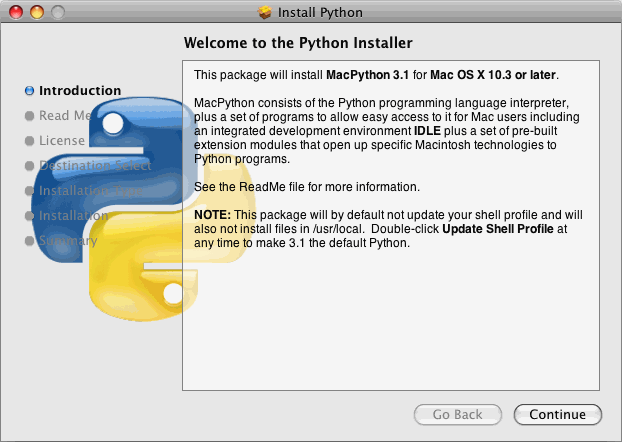
\includegraphics[width=0.5\textwidth]{macInstalacion1.png}
\caption{Bienvenida a la instalación}\label{figm01}
  \end{center}
\end{figure}

La primera página (figura~\ref{figm01}) que muestra el programa de instalación describe de forma concisa qué es Python, y remite al fichero \codigo{ReadMe.txt} (que seguramente no te leíste ¿verdad?) por si deseas conocer más detalles.

Pulsa el botón \codigo{Continue} para avanzar en la instalación.

\begin{figure}[!h]
  \begin{center}
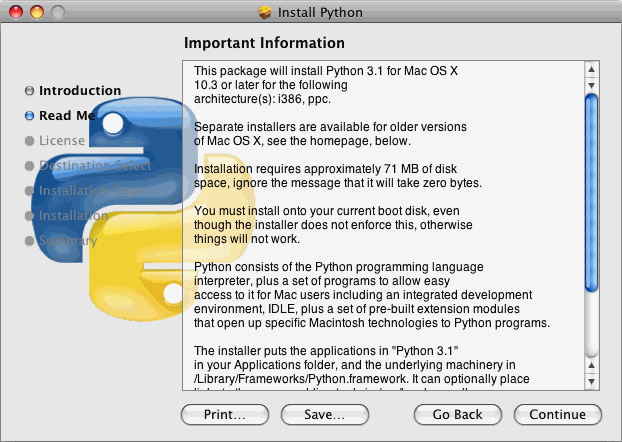
\includegraphics[width=0.5\textwidth]{macInstalacion2.png}
\caption{Información importante}\label{figm02}
  \end{center}
\end{figure}

La siguiente pantalla (figura~\ref{figm02}) muestra información importante: Python necesita que tengas instalado Mac OS X 10.3 o superior. Si estás ejecutando una versión de Mac OS X 10.2 o anterior, deberías actualizar tu ordenador a última versión. Una de las razones más convincentes, es que Apple ya no proporciona actualizaciones de seguridad para tu versión del sistema operativo, por lo que tu ordenadores está en riesgo cada vez que está conectado a Internet. Otra razón, no menos convincente, es que no puedes ejecutar Python 3.

Pulsa el botón \codigo{Continue} para avanzar en la instalación.

\begin{figure}[!h]
  \begin{center}
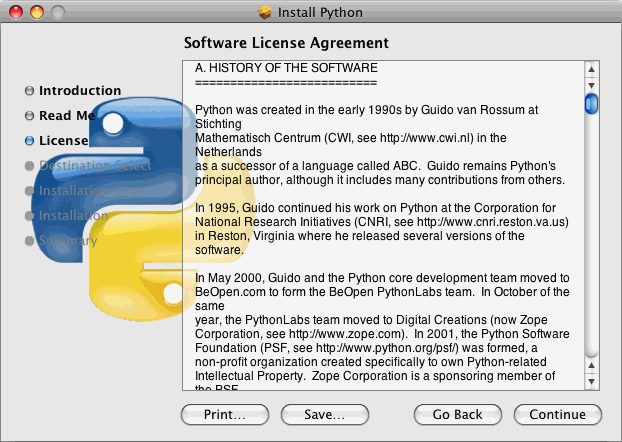
\includegraphics[width=0.5\textwidth]{macInstalacion3.png}
\caption{Licencia}\label{figm03}
  \end{center}
\end{figure}

Como todos los buenos instaladores, lo siguiente que el instalador de Python muestra es la pantalla de aceptación de la licencia (figura~\ref{figm03}). Python es Open Source (software de fuentes abiertas) cuya licencia cuenta con la aprobación de \href{http://opensource.org/licenses/}{la iniciativa de Código Abierto}. Python cuenta con un cierto número de propietarios y patrocinadores a lo largo de su historia, cada uno de los cuales ha dejado su marca en la licencia. Pero el resultado final es este: Python es Código Abierto, y puedes usarlo en cualquier plataforma, para lo que desees, sin necesidad de pagar ningún canon, ni obligación, ni nada a cambio.

Pulsa el botón \codigo{Continue} de nuevo para avanzar en la instalación.

\begin{figure}[!h]
  \begin{center}
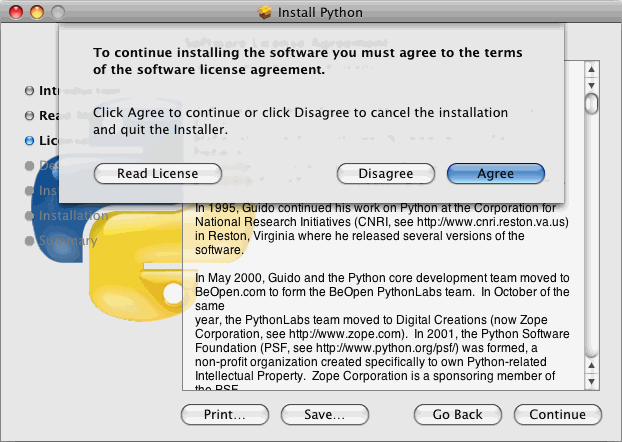
\includegraphics[width=0.5\textwidth]{macInstalacion4.png}
\caption{Aceptación de la Licencia}\label{figm04}
  \end{center}
\end{figure}

Debido a las peculiaridades del proceso de instalación estándar de Apple, es necesario que aceptes la licencia (figura~\ref{figm04}) para que el instalador te permita continuar. Puesto que Python es Código Abierto, en realidad estás aceptando una licencia que te garantiza derechos adicionales, en lugar de quitártelos.

Pulsa el botón \codigo{Agree} para continuar.

La siguiente pantalla (figura~\ref{figm05}) te permite modificar la ubicación en la que se efectuará la instalación. \textbf{Debes} instalar Python en el disco de arranque, pero debido a ciertas limitaciones en el instalador, éste no te obliga a ello, por lo que ¡ten cuidado!. En realidad, yo nunca he tenido la necesidad de cambiar la ubicación de instalación, por ello, salvo causa justificada, acepta la ubicación sugerida por el instalador.

\begin{figure}[!h]
  \begin{center}
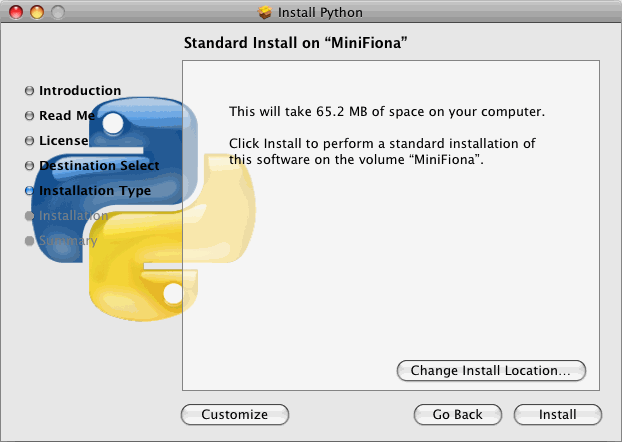
\includegraphics[width=0.5\textwidth]{macInstalacion5.png}
\caption{Selección de la ubicación}\label{figm05}
  \end{center}
\end{figure}

Desde esta pantalla también puedes modificar la instalación con el fin de que no se instalen algunas funcionalidades. Si quieres hacer esto pulsa el botón \codigo{Customize}, en caso contrario pulsa el botón \codigo{Instalar}.

\begin{figure}[!h]
  \begin{center}
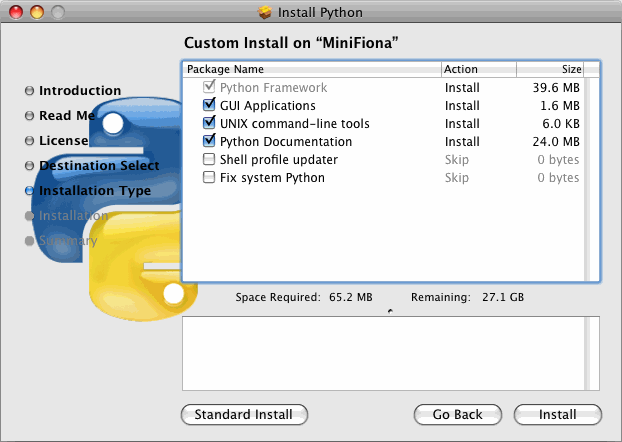
\includegraphics[width=0.5\textwidth]{macInstalacion6.png}
\caption{Personalización de la instalación}\label{figm06}
  \end{center}
\end{figure}

Si eliges una instalación personalizada (has pulsado el botón \codigo{Customize}), el instalador te muestra (figura~\ref{figm06}) una pantalla con una lista de características:

\begin{itemize}
\item \textbf{Python Framework}. Es el núcleo de Python, por lo que está seleccionado y deshabilitado con el fin de que no puedas cambiarlo.
\item \textbf{Aplicaciones GUI} incluye \codigo{IDLE}, la consola interactiva gráfica de Python que usaremos a lo largo de todo el libro. Te recomiendo encarecidamente que mantengas esta opción seleccionada.
\item \textbf{Herramientas de línea de comandos}, que incluyen la aplicación \codigo{python3}. También te recomiendo que mantegas esta opción seleccionada.
\item \textbf{Documentación de Python}, que contiene mucha de la información disponible en \href{http://docs.python.org/}{docs.python.org}. Muy recomendables si tienes previsto estar desconectado de Internet.
\item \textbf{Actualizador del perfil de la consola}, que controla si actualizas tu perfil de consola (utilizado por la aplicación \codigo{Terminal.app}) con el fin de que la versión de Python que estás instalando se encuentre en el camino de búsqueda de la consola. Para los propósitos de este libro, esta opción no es necesario que la instales.
\item \textbf{Actualizar la versión de Python del sistema}. Esta opción no debería modificarse. Le dice a tu ordenador Mac que utilice Python 3 como versión por defecto para todos los scripts, incluido aquellos que vienen con el sistema operativo. Seleccionar esta opción podría producir efectos muy negativos en tu sistema, puesto que la mayor parte de los scripts del sistema operativo están escritos para Python 2, y pueden fallar en Python 3.
\end{itemize}

Pulsa el botón \codigo{Install} para continuar.

\begin{figure}[!h]
  \begin{center}
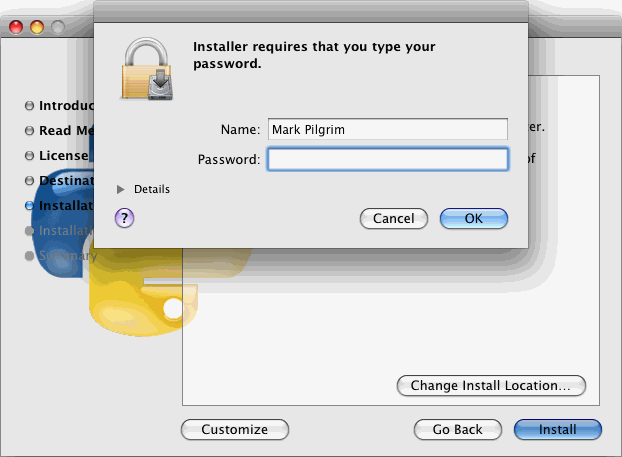
\includegraphics[width=0.5\textwidth]{macInstalacion7.png}
\caption{Solicitando derechos administrativos}\label{figm07}
  \end{center}
\end{figure}

Debido a que el instalador copia archivos binarios en \codigo{/usr/local/bin/}, antes de iniciar dicha copia se solicitan permisos de administrador mediante una pantalla (figura~\ref{figm07}) en la que hay que teclear la clave del administrador del sistema. No es posible instalar Python en Mac sin disponer de las credenciales de administrador.

Pulsa el botón \codigo{OK} para comenzar la instalación.

\begin{figure}[!h]
  \begin{center}
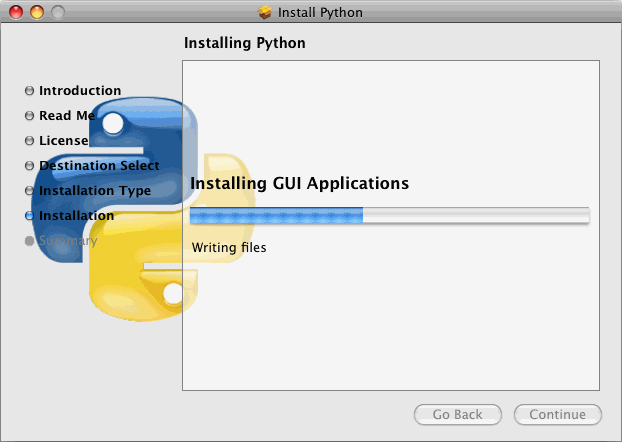
\includegraphics[width=0.5\textwidth]{macInstalacion8.png}
\caption{Instalación}\label{figm08}
  \end{center}
\end{figure}

El instalador mostrará una barra de progreso (figura~\ref{figm08}) mientras se instalan las funcionalidades que hayas seleccionado.

\begin{figure}[!h]
  \begin{center}
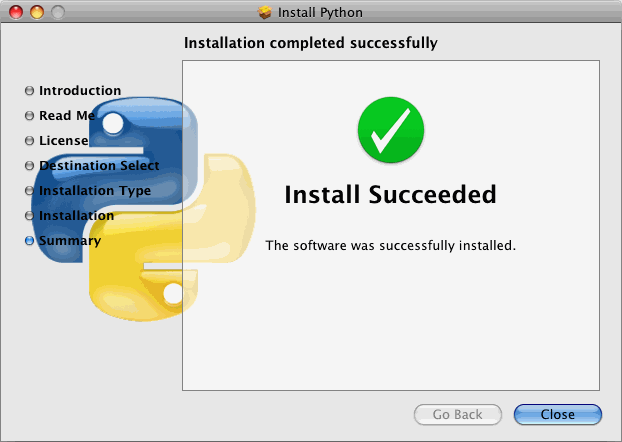
\includegraphics[width=0.5\textwidth]{macInstalacion9.png}
\caption{Fin de la instalación}\label{figm09}
  \end{center}
\end{figure}

Si todo va bien, el instalador mostrará en pantalla (figura~\ref{figm09}) una marca verde para indicar que la instalación de ha completado satisfactoriamente.

Pulsa el botón \codigo{Close} para salir del instalador.

\begin{figure}[!h]
  \begin{center}
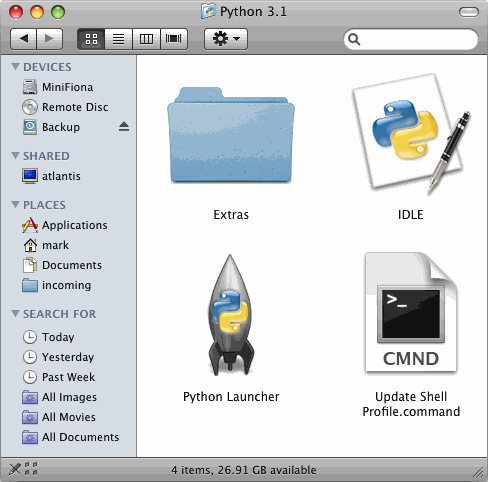
\includegraphics[width=0.5\textwidth]{macInstalacion10.png}
\caption{Carpeta Python}\label{figm010}
  \end{center}
\end{figure}

Si no has cambiado la ubicación de la instalación, \codigo{Python 3.1.*} se habrá instalado en una carpeta denominada \codigo{Python 3.1} (figura~\ref{figm010}) dentro de la carpeta \codigo{/Aplications}. El elemento más importante en ella es \codigo{IDLE}, que es la consola gráfica interactiva de Python.

Haz doble click con el cursor sobre \codigo{IDLE} para ejecutar la consola de Python.

\begin{figure}[!h]
  \begin{center}
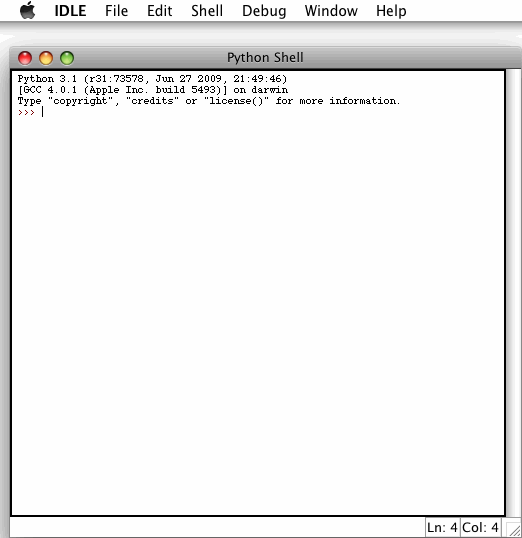
\includegraphics[width=0.5\textwidth]{macInstalacion11.png}
\caption{Consola gráfica}\label{figm011}
  \end{center}
\end{figure}

La mayor parte del tiempo la pasarás explorando Python mediante el uso de esta consola (figura~\ref{figm011}). Los ejemplos de este libro asumen que eres capaz de ejecutar esta consola en todo momento.

Continúa en el apartado~\ref{sec:shell}

\section{Instalación en Ubuntu Linux}

Las diferentes distribuciones existentes hoy día de Linux suelen disponer de vastos repositorios de aplicaciones listas para instalar de forma sencilla. Los detalles exactos varían en función de la distribución de Linux. En Ubuntu Linux, la forma más sencilla de instalar Python 3 consiste en usar la opción \codigo{Añadir y quitar...} del menú de \codigo{Aplicaciones} (figura~\ref{figu00}).

\begin{figure}[!h]
  \begin{center}
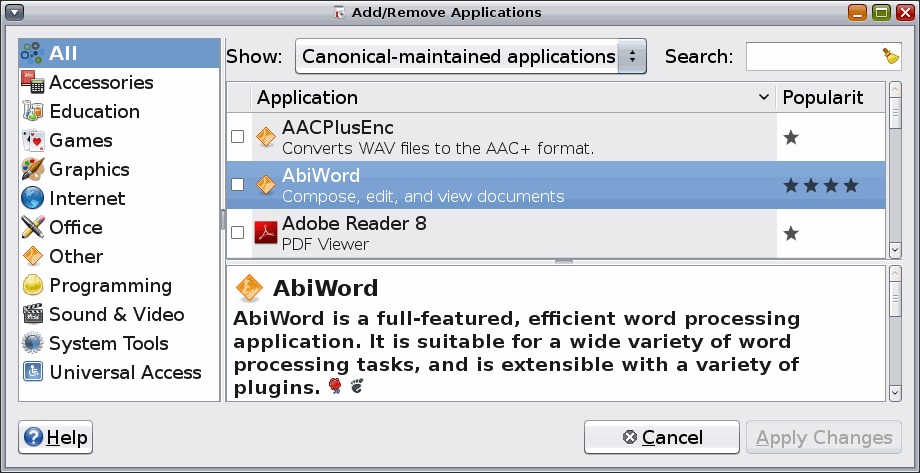
\includegraphics[width=0.6\textwidth]{ubuInstalacion0.png}
\caption{Añadir/Quitar aplicaciones}\label{figu00}
  \end{center}
\end{figure}

Cuando ejecutas por primera vez el programa para \codigo{Añadir/Quitar} aplicaciones, se muestra una lista de aplicaciones preseleccionadas en diferentes categorías. Algunas ya se encuentran instaladas en tu ordenador, pero la mayoría no. Puesto que este repositorio consta de más de 10.000 aplicaciones, encontrar la que se desea puede ser difícil, para facilitar la labor es posible aplicar diferentes filtros que limitan las aplicaciones que se muestran en la lista de pantalla. El filtro por defecto es ``aplicaciones mantenidas por Canonical'' que es el pequeño subconjunto formado por aquellas apliicaciones que se mantienen oficialmente por parte de Canonical, la compañía que distribuye y mantiene Ubuntu Linux.

Como Python 3 no está en este subconjunto de aplicaciones, el primer paso es desplegar los filtros (Mostrar:) y seleccionar \codigo{Todas las aplicaciones libres} (figura~\ref{figu01}).

\begin{figure}[!h]
  \begin{center}
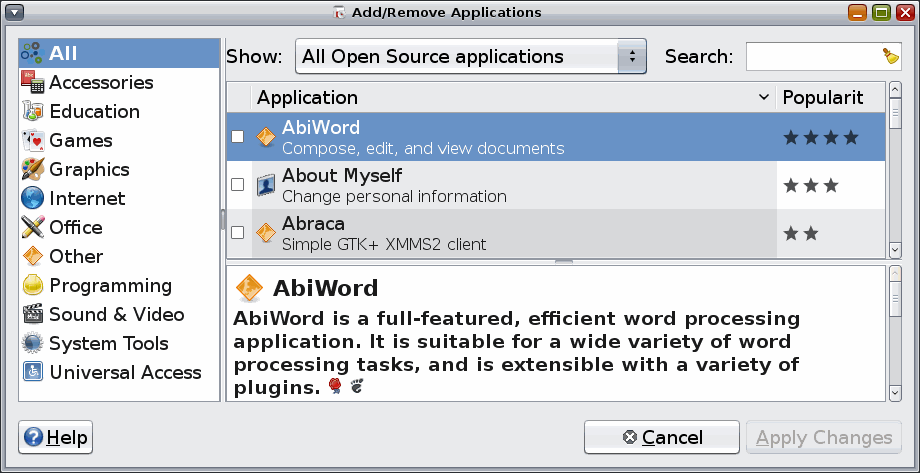
\includegraphics[width=0.6\textwidth]{ubuInstalacion1.png}
\caption{Todas las aplicaciones libres}\label{figu01}
  \end{center}
\end{figure}

Después puedes filtrar aún más utilizando la caja de texto de búsqueda con el fin de buscar el texto \codigo{Python 3} (figura~\ref{figu02}).

\begin{figure}[!h]
  \begin{center}
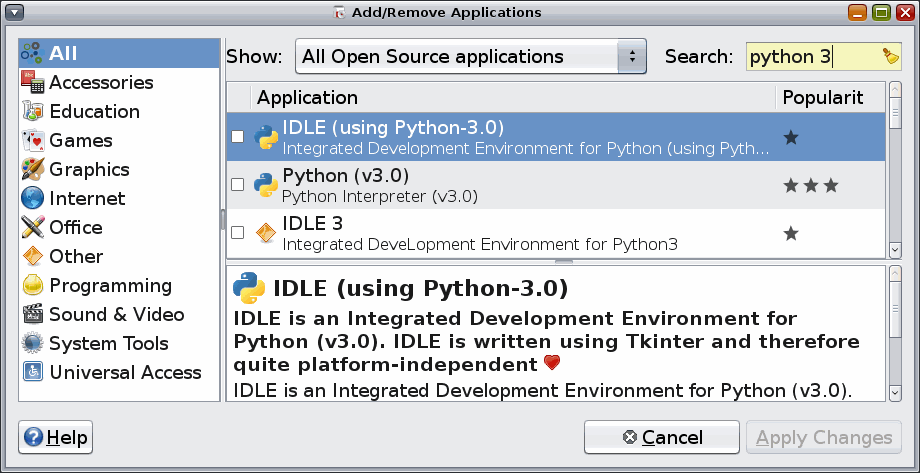
\includegraphics[width=0.6\textwidth]{ubuInstalacion2.png}
\caption{Búsqueda de aplicaciones relacionadas con Python 3}\label{figu02}
  \end{center}
\end{figure}

Ahora la lista de aplicaciones que se muestran se limita a aquellas que, de algún modo, incluyen la cadena \codigo{Python 3}. Ahora debes marcar dos paquetes. El primero es \codigo{Python (v3.0)}. Que contiene el intérprete de Python 3.

\begin{figure}[!h]
  \begin{center}
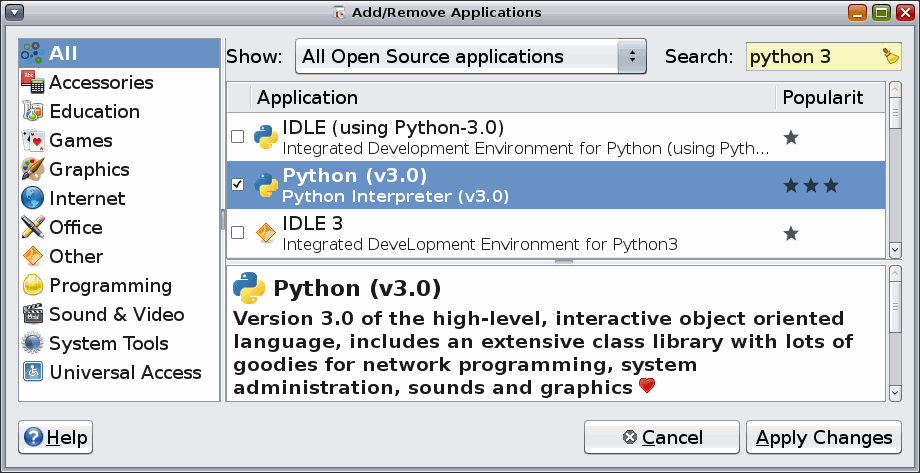
\includegraphics[width=0.6\textwidth]{ubuInstalacion3.png}
\caption{Selección del paquete Python 3}\label{figu03}
  \end{center}
\end{figure}

El segundo paquete que hay que marcar se encuentra inmediatamente delante, \codigo{IDLE (usando Python 3.0)}, que es la consola gráfica que usaremos a lo largo de todo el libro (figura~\ref{figu04}).

\begin{figure}[!h]
  \begin{center}
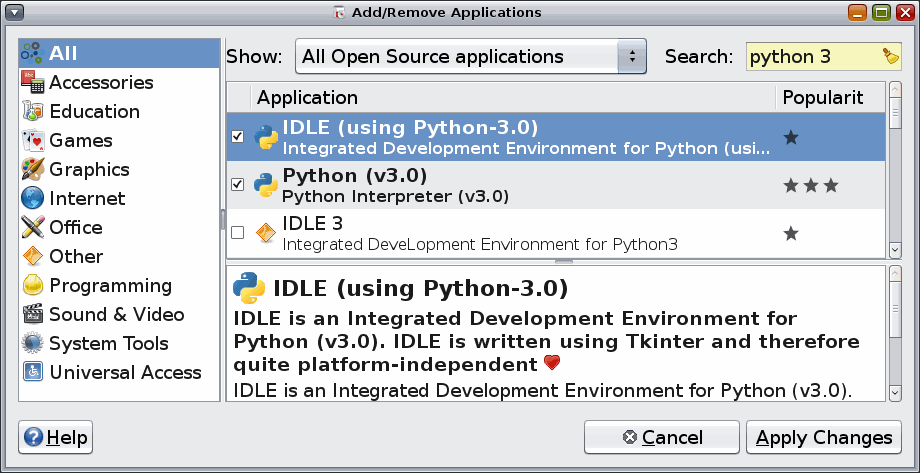
\includegraphics[width=0.6\textwidth]{ubuInstalacion4.png}
\caption{Selección del paquete IDLE}\label{figu04}
  \end{center}
\end{figure}

Una vez hayas seleccionado los dos paquetes, pulsa el botón \codigo{Aplicar cambios} para continuar.

\begin{figure}[!h]
  \begin{center}
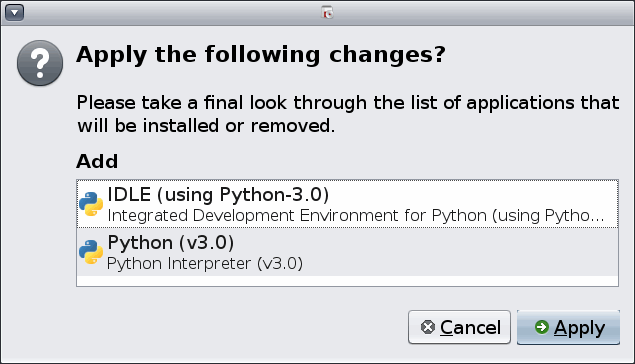
\includegraphics[width=0.6\textwidth]{ubuInstalacion5.png}
\caption{Confirmación}\label{figu05}
  \end{center}
\end{figure}

El gestor de paquetes solicitará que confirmes que quieres instalar tanto \codigo{IDLE (usando Python 3.0)} como \codigo{Python (3.0)} (figura~\ref{figu05}).

Pulsa el botón \codigo{Aplicar} para continuar.

\begin{figure}[!h]
  \begin{center}
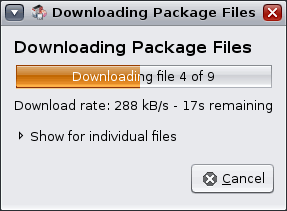
\includegraphics[width=0.5\textwidth]{ubuInstalacion6.png}
\caption{Descarga de paquetes}\label{figu06}
  \end{center}
\end{figure}

El gestor de paquetes te pedirá que te identifiques con la clave de usuario para acceder a los privilegios administrativos que permiten instalar aplicaciones. Una vez hecho esto, el gestor de paquetes mostrará una pantalla (figura~\ref{figu06}) con el grado de avance de la instalación mientras se descargan los paquetes seleccionados del repositorio de Internet de Ubuntu Linux.

\begin{figure}[!h]
  \begin{center}
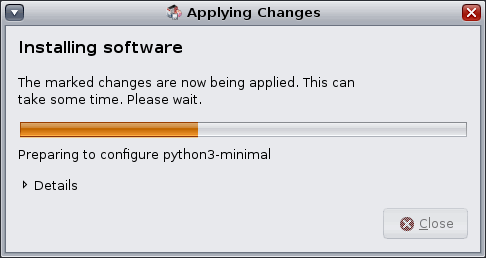
\includegraphics[width=0.5\textwidth]{ubuInstalacion7.png}
\caption{Descarga de paquetes}\label{figu07}
  \end{center}
\end{figure}

Cuando los paquetes se hayan descargado, el instalador iniciará automáticamente el proceso de instalación en tu ordenador (figura~\ref{figu07}).

\begin{figure}[!h]
  \begin{center}
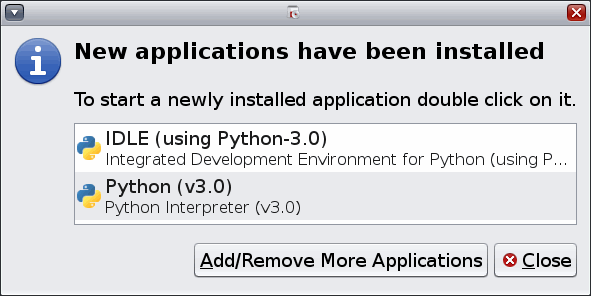
\includegraphics[width=0.5\textwidth]{ubuInstalacion8.png}
\caption{Instalación finalizada}\label{figu08}
  \end{center}
\end{figure}

Si todo va bien, el gestor de paquetes confirmará que ambos paquetes se instalaron satisfactoriamente (figura~\ref{figu08}). Desde esta pantalla puedes ejecutar directamente \codigo{IDLE} haciendo doble click sobre él. O puedes pulsar el botón \codigo{Cerrar} para finalizar el gestor de paquetes.

En cualquier caso, puedes lanzar la consola gráfica de Python siempre que quieras seleccionando \codigo{IDLE} en el submenú \codigo{Programación} del menú de \codigo{Aplicaciones}.

\begin{figure}[!h]
  \begin{center}
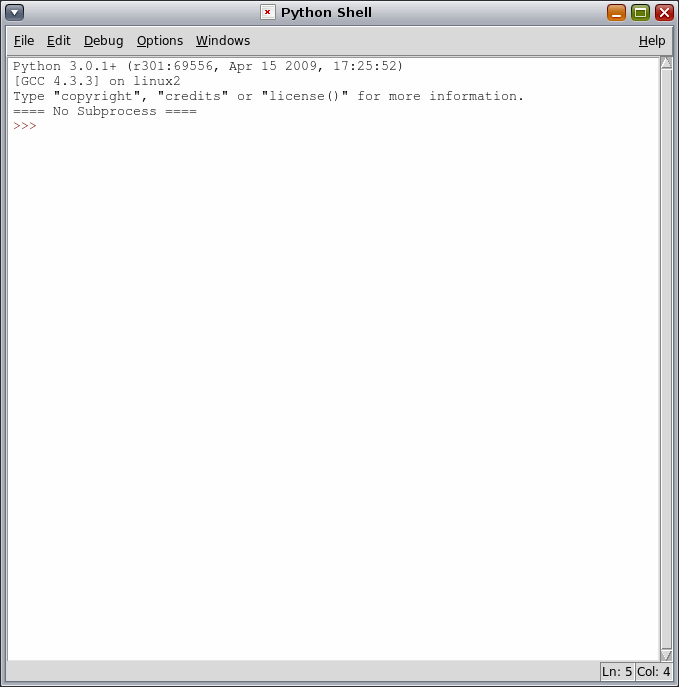
\includegraphics[width=0.5\textwidth]{ubuInstalacion9.png}
\caption{Consola de Python en Ubuntu Linux}\label{figu09}
  \end{center}
\end{figure}

Es en la consola de Python (figura~\ref{figu09}) donde pasarás la mayor parte del tiempo explorando Python. Los ejemplos de este libro asumen que eres capaz de ejecutar la consola de Python siempre que sea necesario.

Continúa en el apartado~\ref{sec:shell}

\section{Instalación en otras plataformas}

Python 3 está disponible en otras muchas plataformas. En particular, está disponible prácticamente en todas las distribuciones Linux, BSD y Sun Solaris. Por ejemplo, RedHat Linux utiliza el gestor de paquetes \codigo{yum}; FreeBSD tiene su propia colección de \href{http://www.freebsd.org/ports/}{paquetes}, y Solaris tiene el gestor de paquetes \codigo{pkgadd} y otros. Una rápida búsqueda en Internet de los términos Python 3 + emph{tu sistema operativo} te mostrará si existe un paquete de Python 3 disponible para tu sistema, y cómo instalarlo.

\section{Uso de la consola interactiva de Python}\label{sec:shell}

En la consola interactiva de Python puedes explorar la sintaxis del lenguaje, solicitar ayuda interactiva sobre las sentencias del lenguaje, y depurar programas cortos.

La consola gráfica (denominada \codigo{IDLE}) también proporciona un editor de textos bastante decente que resalta mediante colores la sintaxis del lenguaje Python. Si no tienes aún un editor de textos de tu elección, puedes darle una oportunidad a \codigo{IDLE}.

¡Vamos a comenzar! La shell de Python es un estupendo lugar para comenzar a \emph{jugar} con el lenguaje Python de forma interactiva.  A lo largo de este libro verás un montón de ejemplos como este:

\begin{listing}
\begin{verbatim}
>>> 1 + 1
2
\end{verbatim}
\end{listing}

Los tres símbolos de \emph{mayor que}, \codigo{$>>>$}, representan el \emph{prompt}\footnote{Nota del Traductor: El prompt es el indicador que usa una consola, en este caso la consola de Python, para que el usuario sepa que puede teclear alguna sentencia. Como el uso de la palabra \emph{prompt} está tan extendido para este concepto, y no existe uno en español de amplio uso, en este libro se utilizará sin traducir.} de Python. No teclees nunca estos tres caracteres. Se muestran para que sepas que este ejemplo se debe teclear en la consola de Python.

Lo que tienes que teclear es \codigo{1 + 1}.  En la consola puedes teclear cualquier expresión o sentencia válida del lenguaje. ¡No seas tímido, no muerde! Lo peor que puede pasarte es que Python muestre un mensaje de error, si tecleas algo que no entiende. Las sentencias se ejecutan inmediatamente (después de que pulses la tecla \codigo{INTRO}); las expresiones se calculan en el momento, y la consola imprime en pantalla el resultado.

\codigo{2} es el resultado de la expresión. Como \codigo{1 + 1} es una expresión válida en el lenguaje Python, al pulsar la tecla \codigo{INTRO} Python evalúa la expresióne imprime el resultado, que en este caso es \codigo{2}.

Vamos a probar otro ejemplo.

\begin{listing}
\begin{verbatim}
>>> print('¡Hola mundo!')
¡Hola mundo!
\end{verbatim}
\end{listing}

Muy sencillo, ¿no?

Pero hay muchas otras cosas que puedes hacer en la consola de Python. Si en algún momento te bloqueas ---no recuerdas una sentencia, o no recuerdas los argumentos que debes pasar a una función determinada--- puedes obtener ayuda en la propia consola. Simplemente teclea \codigo{help} y pulsa \codigo{ENTER}.

\begin{listing}
\begin{verbatim}
>>> help
Type help() for interactive help, or help(object) for help about object.
\end{verbatim}
\end{listing}

Exiten dos modos de ayuda:
\begin{itemize}
\item Puedes solicitar ayuda de un objeto concreto, lo que muestra la documentación del mismo y vuelve al \codigo{prompt} de la consola de Python. 
\item También puedes entrar en el \emph{modo ayuda}, en el que en lugar de evaluar expresiones de Python, puedes teclear palabras reservadas del lenguaje o nombres de sentencias y la consola imprime lo que sepa sobre ellas.
\end{itemize}

Para entrar en el modo interactivo de ayuda teclea \codigo{help()} y pulsa \codigo{INTRO}.

\begin{listing}
\begin{verbatim}
>>>help()

Welcome to Python 3.0!  This is the online help utility.

If this is your first time using Python, you should definitely check out
the tutorial on the Internet at http://docs.python.org/tutorial/.

Enter the name of any module, keyword, or topic to get help on writing
Python programs and using Python modules.  To quit this help utility and
return to the interpreter, just type "quit".

To get a list of available modules, keywords, or topics, type "modules",
"keywords", or "topics".  Each module also comes with a one-line summary
of what it does; to list the modules whose summaries contain a given word
such as "spam", type "modules spam".

help>
\end{verbatim}
\end{listing}

Observa que ahora el prompt cambia de \codigo{$>>>$} a \codigo{help$>$}. Este cambio sirve para recordarte que te encuentras en el modo de ayuda interactiva. Ahora puedes teclear cualquier palabra reservada, sentencia, nombre de módulo, nombre de función ---casi cualquier cosa que Python entienda--- y leer la documentación que haya disponible sobre el tema tecleado.

\begin{listing}
\begin{verbatim}
help> print

Help on built-in function print in module builtins:

print(...)
    print(value, ..., sep=' ', end='\n', file=sys.stdout)
    
    Prints the values to a stream, or to sys.stdout by default.
    Optional keyword arguments:
    file: a file-like object (stream); defaults to the current sys.stdout.
    sep:  string inserted between values, default a space.
    end:  string appended after the last value, default a newline.
help> Papaya
no Python documentation found for 'Papaya'
\end{verbatim}
\end{listing}
\begin{listing}
\begin{verbatim}
help> quit

You are now leaving help and returning to the Python interpreter.
If you want to ask for help on a particular object directly from the
interpreter, you can type "help(object)".  Executing "help('string')"
has the same effect as typing a particular string at the help> prompt.

>>>
\end{verbatim}
\end{listing}

En el ejemplo anterior se obtiene en primer lugar la documentación sobre la función print. Para ello se ha tecleado en el modo ayuda la palabra \codigo{print} y luego se ha pulsado \codigo{INTRO}. Como resultado se obtiene un texto en el que se muestra el nombre de la función, un breve resumen de la misma, los argumentos de la función y sus valores por defecto. Si la documentación te parece demasiado opaca, no te asustes. Aprenderás lo necesario sobre todos estos conceptos en los próximos capítulos de este libro.

Evidentemente el modo de ayuda no lo sabe todo. Si tecleas algo que no sea una sentencia, módulo, función u otra palabra reservada de Python,el modo de ayuda interactiva mostrará un mensaje indicando que no encuentra documentación alguna para el concepto que hayas tecleado.

Por último, para salir del modo de ayuda únicamente tienes que teclear \codigo{quit} y pulsar \codigo{INTRO}.

El prompt vuelve de nuevo a \codigo{$>>>$} para indicar que has abandonado el modo de ayuda interactiva y que de nuevo te encuentras en la consola de Python.

\codigo{IDLE}, además de servir como consola gráfica de Python, incluye también un editor de textos que conoce el lenguaje Python. Verás cómo usarlo en la sección siguiente.

\section{Editores de texto e IDEs para Python}

\codigo{IDLE} no es el único entorno existente para escribir programas en Python. Aunque es muy útil para comenzar a aprender el lenguaje, muchos desarrolladores prefieren utilizar otros editores de texto o \emph{Entornos Integrados de Desarrollo}\footnote{En inglés se suele hablar de \codigo{IDE}, para referirse a los \emph{Integrated Development Environment}, que son aplicaciones que permiten desarrollar de forma rápida al incluir un editor de textos, compilador, depurador e incluso herramientas de diseño de aplicaciones avanzadas.}. No los voy a abarcar aquí, únicamente comentaré que la comunidad de Python mantiene una lista de \href{http://wiki.python.org/moin/PythonEditors}{editores para el lenguaje Python} sobre diversas plataformas y licencias de software.

También puede ser de interés para ti la lista de \href{http://wiki.python.org/moin/IntegratedDevelopmentEnvironments}{Entornos Integrados de Desarrollo} para Python, aunque aún son pocos los que sirven para Python 3. Uno de ellos es \href{http://pydev.sourceforge.net/}{PyDev}, un plugin para \href{http://eclipse.org/}{Eclipse} que convierte a Eclipse en un completo Entorno Integrado de Desarrollo para Python. Ambos, Eclipse y PyDev, son multiplataforma y de código abierto.

Por la parte comercial, existe un entorno de desarrollo denominado \href{http://www.activestate.com/komodo/}{Komodo IDE}. Tiene una licencia que se paga por cada usuario, pero también ofrece descuento para estudiantes, y una versión con licencia de prueba limitada.

Llevo programando en Python nueve años, yo, para editar los programas, utilizo \href{http://www.gnu.org/software/emacs/}{GNU Emacs} y los depuro en la shell de línea de comando\footnote{Nota del Traductor:En mi caso uso \href{http://www.vim.org}{GVim} y el depurador de consola \href{http://pypi.python.org/pypi/pudb}{pudb}}. No existe un modo correcto de desarrollar en Python. ¡Encuentra lo que mejor se adapte a ti!


% ch1.tex
% This work is licensed under the Creative Commons Attribution-Noncommercial-Share Alike 3.0 New Zealand License.
% To view a copy of this license, visit http://creativecommons.org/licenses/by-nc-sa/3.0/nz
% or send a letter to Creative Commons, 171 Second Street, Suite 300, San Francisco, California, 94105, USA.

\chapter{Tu primer programa en Python}\label{ch:primerprograma}

\noindent
Nivel de dificultad:\difl

\begin{citaCap}
``No entierres tu carga en un santo silencio.\\
¿Tienes un problema? Estupendo. Alégrate, \\
sumérgete en él e investiga.''\\
---\href{http://en.wikiquote.org/wiki/Buddhism}{Ven. Henepola Gunarata}
\end{citaCap}

\section{Inmersión}

Los libros sobre programación suelen comenzar con varios capítulos sobre los fundamentos y van, poco a poco, avanzando hasta llegar a hacer programas útiles. Vamos a saltarnos todo eso. Lo primero que vamos a ver es un programa Python completo. Probablemente no tenga ningún sentido para ti. No te preocupes por eso, vamos a diseccionarlo línea por línea. Primero léelo y trata de interpretarlo.

\begin{lstlisting}[mathescape=True]
# parahumanos.py

SUFIJOS = {1000: ['KB', 'MB', 'GB', 'TB', 'PB', 'EB', 'ZB', 'YB'],
           1024: ['KiB', 'MiB', 'GiB', 'TiB', 'PiB', 'EiB', 'ZiB', 
                  'YiB']}

def tamanyo_aproximado(tamanyo, un_kilobyte_es_1024_bytes=True):
    '''Convierte un tama$\til{n}$o de fichero en formato legible por personas

    Argumentos/par$\ac{a}$metros:
    tamanyo -- tama$\til{n}$o de fichero en bytes
    un_kilobyte_es_1024_bytes -- si True (por defecto), 
                                 usa m$\ac{u}$ltiplos de 1024
                                 si False, usa m$\ac{u}$ltiplos de 1000

    retorna: string

    '''
    if tamanyo < 0:
        raise ValueError('el n$\ac{u}$mero debe ser no negativo')

    multiplo = 1024 if un_kilobyte_es_1024_bytes else 1000
    for sufijo in SUFIJOS[multiplo]:
        tamanyo /= multiplo
        if tamanyo < multiplo:
            return '{0:.1f} {1}'.format(tamanyo, sufijo)

    raise ValueError('n$\ac{u}$mero demasiado grande')

if __name__ == '__main__':
    print(tamanyo_aproximado(1000000000000, False))
    print(tamanyo_aproximado(1000000000000))

\end{lstlisting}

Antes de analizarlo paso a paso vamos a ejecutar el programa en la línea de comandos. En Linux o en Mac debes teclear: \codigo{python3 parahumanos.py}\footnote{Para que funcione correctamente debes moverte al directorio en el que esté grabado el fichero \codigo{parahumanos.py}.}. El resultado será parecido a lo siguiente:

\begin{lstlisting}
tu_usuario@tu_ordenador:~/inmersionEnPython3$\$$ python3 parahumanos.py
1.0 TB
931.3 GiB
\end{lstlisting}

En Windows debes teclear lo mismo: \codigo{python3 parahumanos.py}, únicamente varía la forma del prompt de la consola. El resultado será parecido a:

\begin{lstlisting}
C:\\inmersionenpython3:> python3 parahumanos.py
1.0 TB
931.3 GiB
\end{lstlisting}

¿Qué ha pasado? Acabas de ejecutar tu primer programa Python. Has ejecutado el intérprete de Python en la línea de comandos (\codigo{python3}), y le has pasado como parámetro el nombre del fichero de script (\codigo{parahumanos.py}) que querías ejecutar. 

El fichero de script, a su vez, define una única función de python, la función \codigo{tamnyo\_aproximado}, que toma como parámetros un tamaño de fichero con una precisión de bytes y calcula el tamaño en una unidad mayor en la que el valor quede más \emph{bonito}, a cambio, el resultado es aproximado. (El funcionamiento del Explorador de Windows; del Finder de Mac OS X, o de Nautilus, Dolphin o Thunar de Linux es muy parecido. Si muestras en cualquiera de ellos una carpeta de documentos en modo detalle, de forma que se vean en diferentes columnas, el icono del documento, nombre, tamaño, tipo, fecha de última modificación, etc. Observarás que si un documento determinado ocupa 1093 bytes, en la columna de tamaño no dirá eso, sino que dirá algo así como 1 KB. Esto es lo que hace la función \codigo{tamanyo\_aproximado})

Las líneas de código \codigo{print(tamanyo\_aproximado(\emph{argumentos}))} del final del script, líneas 31 y 32, son dos llamadas a funciones ---primero se llama a la función \codigo{tamanyo\_aproximado()} pasándole unos parámetros (también llamados argumentos), esta función se ejecuta y devuelve un resultado que, posteriormente, se pasa como parámetro a la función \codigo{print()}. Todo ello en la misma línea.

La función \codigo{print()} es interna del lenguaje Python\footnote{En inglés \codigo{built-in}.}; nunca verás una declaración explícita de ella. La puedes usar cuando quieras, en cualquier parte de un programa Python\footnote{Existen montones de funciones internas del lenguaje, y muchas más que están separadas en \emph{módulos}. Lo veremos poco a poco, ten paciencia, pequeño saltamontes.}.

¿Porqué la ejecución del script en la línea de comandos retorna siempre la misma respuesta? Lo veremos más adelante. Primero vamos a ver el funcionamiento de la función \codigo{tamanyo\_aproximado()}.

\section{Declaración de funciones}

Python dispone de funciones como la mayoría de los lenguajes, pero no tiene ficheros de cabecera como \codigo{c++} o secciones de \codigo{interface/implementation} como en Pascal. En Python únicamente hay que declarar la función, como en el siguiente ejemplo:

\begin{lstlisting}
def tamanyo_aproximado(tamanyo, un_kilobyte_es_1024_bytes=True):
\end{lstlisting}

La palabra reservada \codigo{def} inicia la declaración de la función, seguida del nombre que le quieres dar a la misma, seguida de los parámetros de la función entre paréntesis. Separándolos por comas en caso de que sean varios parámetros.

\cajaTexto{En Python cuando necesitas una función, solamente tienes que declararla.}

Observa también que, en Python, las funciones no definen un tipo de datos de retorno. No se especifica el tipo de datos del valor que retornan las funciones. Es más, ni siquiera se especifica si se retorna o no un valor. 

En realidad, todas las funciones de Python tienen un valor de retorno; si dentro del código de la función se ejecuta una sentencia \codigo{return}, el valor que acompaña a la sentencia será el valor de retorno, en caso contrario se retorna el valor \codigo{None}, que es la forma de expresar el vacío (\codigo{null}) en Python.

\begin{quote}
En algunos lenguajes, las funciones que retornan un valor se declaran con la palabra \codigo{function}, y las subrutinas que no retornan un valor con la palabra \codigo{sub}. En Python no existen las subrutinas. Todas son funciones, todas las funciones devuelven un valor (\codigo{None} si tú no devuelves algo expresamente con la palabra reservada \codigo{return}) y todas las funciones comienzan con la palabra \codigo{def}.
\end{quote}

La función \codigo{tamanyo\_aproximado()} recibe dos parámetros o argumentos, ---\codigo{tamanyo} y \codigo{un\_kilobyte\_es\_1024\_bytes}--- pero ninguno de ellos especifica un tipo de datos. En Python, las variables nunca se tipifican explícitamente, Python deduce y  mantiene el tipo de datos de la variable de forma interna según el valor que tenga asignado la misma.

\begin{quote}
En Java y otros lenguajes con tipificación estática, debes especificar el tipo de datos de los parámetros y valor de retorno de cada función. En Python nunca especificas el tipo de datos de nada de forma explícita. Python mantiene el rastro de los tipos de datos de forma interna basándose en los valores que asignes a las variables.
\end{quote}

\subsection{Parámetros opcionales y con nombre}

Python permite que los parámetros de una función tengan valores por defecto; si la función se llama (para ejecutarla) si indicar el parámetro Python usará el valor por defecto para asignarlo al parámetro que no se ha especificado en la llamada a la función. Asimismo, los parámetros se pueden pasar en la llamada en cualquier orden si se utilizan parámetros con nombre.

Veamos de nuevo la declaración de la función \codigo{tamanyo\_aproximado()}.

\begin{lstlisting}
def tamanyo_aproximado(tamanyo, un_kilobyte_es_1024_bytes=True):
\end{lstlisting}

El segundo parámetro \codigo{un\_kilobyte\_es\_1024\_bytes}, especifica un valor por defecto igual a \codigo{True}. Como consecuencia, este parámetro pasa a ser \emph{opcional}; puedes llamar a la función sin pasarlo en los paréntesis. Python se comportará como si lo hubieras llamado con el valor \codigo{True} como segundo parámetro.

Veamos el final del script\footnote{En Python se les suele llamar también \emph{script} a los ficheros con el código fuente de los programas.}:


\begin{lstlisting}
if __name__ == '__main__':
    print(tamanyo_aproximado(1000000000000, False))
    print(tamanyo_aproximado(1000000000000))
\end{lstlisting}

\begin{enumerate}
\item La primera llamada a la función (línea 2) utiliza dos parámetros. Durante la ejecución de la función \codigo{tamanyo\_aproximado} \codigo{un\_kilobyte\_es\_1024\_bytes} tendrá el valor \codigo{False}, que es lo que se pasa como segundo parámetro en la llamada a la función.

\item La segunda llamada a la función (línea 3) utiliza un único parámetro. Pero Python no se queja ya que el segundo es opcional. Como no se especifica, el segundo parámetro utiliza su valor por defecto \codigo{True}, de acuerdo a lo que se definió en la declaración de la función.
\end{enumerate}

También puedes pasar los valores a una función utilizando nombres. Prueba lo siguiente en la consola:

\begin{lstlisting}
>>> from parahumanos import tamanyo_aproximado
>>> tamanyo_aproximado(4000, un_kilobyte_es_1024_bytes=False)
'4.0 KB'
>>> tamanyo_aproximado(tamanyo=4000, un_kilobyte_es_1024_bytes=False)
'4.0 KB'
>>> tamanyo_aproximado(un_kilobyte_es_1024_bytes=False, tamanyo=4000)
'4.0 KB'
>>> tamanyo_aproximado(un_kilobyte_es_1024_bytes=False, 4000)
SyntaxError: non-keyword arg after keyword arg (<pyshell#4>, line 1)
>>> tamanyo_aproximado(tamanyo=4000, False)
SyntaxError: non-keyword arg after keyword arg (<pyshell#5>, line 1)
>>> 
\end{lstlisting}

\begin{enumerate}
\item \emph{Línea 2:} Llama a la función \codigo{tamnyo\_aproximado()} pasándole \codigo{4000} al primer parámetro (\codigo{tamanyo}) y el valor \codigo{False} en el denominado \codigo{un\_kilobyte\_es\_1204\_bytes} (En este caso coincide que el parámetro con nombre se está pasando en la segunda posición y también está declarado en la función como segundo parámetro, pero esto es simplemente una coincidencia).

\item \emph{Línea 4:} Llama a la función \codigo{tamanyo\_aproximado()} pasándole \codigo{4000} al parámetro denominado \codigo{tamanyo} y \codigo{False} al parámetro denominado \codigo{un\_kilobyte\_es\_1024\_bytes} (Estos parámetros coinciden en orden con los de la declaración de la función, pero vuelve a ser una simple coincidencia).

\item \emph{Línea 6:} Llama a a la función \codigo{tamanyo\_aproximado()} paándole \codigo{False} al parámetro denominado \codigo{un\_kilobyte\_es\_1024\_bytes} y \codigo{4000} al parámetro denominado \codigo{tamanyo} (Esta es la utilidad de usar nombres en las llamadas a una función, poder pasarlos en cualquier orden, e incluso no pasar alguno de los existentes para que tomen valores por defecto mientras sí que pasas uno de los últimos parámetros de la función).

\item \emph{Línea 8:} Esta llamada a la función falla porque se usa un parámetro con nombre seguido de uno sin nombre (por posición). Esta forma de llamar a la función siempre falla. Python lee la lista de parámetros de izquierda a derecha, en cuanto aparece un parámetro con nombre, el resto de parámetros debe también proporcionarse por nombre. Los primeros pueden ser por posición.

\item \emph{Línea 10:} Esta llamada también falla por la misma razón que la anterior. ¿Te sorprende? Después de todo, el primer parámetro se ha denominado \codigo{tamanyo} y recibe el valor \codigo{4000}, es \emph{obvio} que el valor \codigo{False} debería asignarse al parámetro \codigo{un\_kilobyte\_es\_1024\_bytes}. Pero Python no funciona de esa forma. Tan pronto como lee un parámetro con nombre, todos los parámetros siguientes (a la derecha) tienen que llevar el nombre del parámetro.
\end{enumerate}

\section{Cómo escribir código legible}

No te voy a aburrir con una larga charla sobre la importancia de documentar el código. Solamente decir que el código se escribe una vez pero se lee muchas veces, y que quien más lo va a leer eres tú, seis meses después de haberlo escrito (por ejemplo: cuando ya no te acuerdes de nada pero necesites corregir o añadir algo). Python hace fácil escribir código legible, aprovéchate de ello. Me lo agradecerás dentro de seis meses.

\subsection{Cadenas de texto de documentación}

Puedes documentar una función proporcionándole una cadena de documentación (abreviando se suele hablar de \codigo{docstring}). En este programa, la función \codigo{tamanyo\_aproximado()} tiene una cadena de documentación (\codigo{docstring}):

\noindent\begin{minipage}{\textwidth}
\begin{lstlisting}[mathescape=True]
def tamanyo_aproximado(tamanyo, un_kilobyte_es_1024_bytes=True):
    '''Convierte un tama$\til{n}$o de fichero en formato legible por personas

    Argumentos/par$\ac{a}$metros:
    tamanyo -- tama$\til{n}$o de fichero en bytes
    un_kilobyte_es_1024_bytes -- si True (por defecto), 
                                 usa m$\ac{u}$ltiplos de 1024
                                 si False, usa m$\ac{u}$ltiplos de 1000

    retorna: string

    '''
\end{lstlisting}
\end{minipage}

La comillas triples sirven para escribir cadenas de texto que ocupen más de una línea. Todo lo que se escribe entre las comillas triples forma parte de una única cadena de texto, incluídos los espacios en blanco, retornos de carro, saltos de línea y otras comillas \emph{sueltas}. Este tipo de cadenas de texto lo puedes utilizar donde quieras dentro del código Python, pero normalmente se utilizan para definir \codigo{docstring} (cadenas de texto de documentación).

\begin{quote}
Las comillas triples son la manera más simple de escribir cadenas de texto que incluyan, a su vez, comillas simples y/o dobles, como cuando en Perl 5 se utiliza \codigo{q/.../}
\end{quote}

\cajaTexto{Todas las funciones se merecen un \emph{docstring} que las explique}

En este ejemplo, todo lo que se encuentra entre las comillas triples es el \codigo{docstring} de la función, que sirve para documentar lo que hace la función. Un \codigo{docstring}, si existe, debe ser lo primero que aparece definido en una función (es decir, se debe encontrar en la primera línea que aparece después de la declaración de la función). Técnicamente no necesitas escribir un \codigo{docstring} para cada función, pero deberías. Sé que lo has escuchado en las clases que programación a las que hayas asistido, pero Python te da un incentivo mayor para que lo hagas: los \codigo{docstring} están disponibles en tiempo de ejecución como un atributo de la función.

\begin{quote}
Muchos entornos integrados de programación (\codigo{IDEs}) utilizan los \codigo{docstring} para proporcionar ayuda y documentación sensible al contexto, de forma que cuando teclees el nombre de una función, aparece su \codigo{docstring} como pista sobre el significado de la función y de sus parámetros. Esto puede ser muy útil, tan útil como explicativos sean los \codigo{docstring} que escribas.
\end{quote}

\section{El camino de búsqueda para \codigo{import}}

Antes de continuar, quiero mencionar brevemente el camino\footnote{En español se usa también \codigo{ruta de búsqueda}. En inglés se usa la palabra \codigo{path} para referirse a este concepto} de búsqueda de las librerías. Cuando importas un módulo, Python busca en varios lugares hasta encontrarlo. En concreto, busca en todos los directorios que se encuentren definidos en la variable \codigo{sys.path}. Como se trata de una \codigo{lista}, puedes verla fácilmente o modificarla con los métodos estándares de manipulación de listas. (Aprenderás a trabajar con listas en el capítulo ~\ref{tiposdedatonativos} sobre Tipos de Dato Nativos).

\noindent\begin{minipage}{\textwidth}

\begin{lstlisting}[mathescape=True]
>>> import sys
>>> sys.path
['', 
 '/usr/lib/python3.0',  
 '/usr/lib/python3.0/plat-linux2',
 '/usr/lib/python3.0/lib-dynload',
 '/usr/lib/python3.0/dist-packages',
 '/usr/local/lib/python3.0/dist-packages']
>>> sys
<module 'sys' (built-in)>
>>> sys.path.insert(0, '/home/jmgaguilera/inmersionenpython3/ejemplos')
>>> sys.path
['/home/jmgaguilera/inmersionenpython3/ejemplos',
 '',
 '/usr/lib/python3.0',
 '/usr/lib/python3.0/plat-linux2',
 '/usr/lib/python3.0/lib-dynload',
 '/usr/lib/python3.0/dist-packages',
 '/usr/local/lib/python3.0/dist-packages']
>>> 

\end{lstlisting}
\end{minipage}

\begin{enumerate}

\item \emph{Línea 1:} Al importar el paquete \codigo{sys} de esta forma, todas sus funciones y atributos quedan a disposición del programador para su uso.

\item \emph{Líneas 2-8:} \codigo{sys.path} es una variable (\codigo{path}) del paquete \codigo{sys} que contiene una lista de los directorios que constituyen el camino de búsqueda (El tuyo será diferente, ya que depende del sistema operativo, de la versión de Python que tengas instalada, y del lugar en el que está instalada). Siempre que se haga un \codigo{import} en el código, Python buscará en estos directorios (por orden), hasta encontrar un fichero cuyo nombre coincida con el valor que se usa en la sentencia \codigo{import} cmás la extensión \codigo{.py}.

\item \emph{Líneas 9-10:} En realidad te he mentido un poco, la realidad es un poco más compleja, no todos los módulos se almacenan en ficheros con extensión \codigo{.py}. Algunos de ellos, como el módulo \codigo{sys} son módulos internos (\codigo{built-in}); no existen en ficheros, están construidos internamente en el propio lenguaje. En la práctica funcionan exactamente igual que los módulos que están en ficheros, la única diferencia es que no existe el código fuente, ¡Porque no están escritos en Python! (El módulo \codigo{sys} está escrito en lenguaje \codigo{c}).

\item \emph{Línea 11:} En \emph{tiempo de ejecución} puedes añadir un nuevo directorio al camino de búsqueda de Python añadiendo un directorio a la variable \codigo{sys.path}, así Python también buscará en él cada vez que intentes importar un módulo. El efecto de este cambio dura mientras se mantenga en ejecución Python. Al finalizar, y volver a entrar en Python, el camino (la variable \codigo{sys.path}) volverá a tener los valores iniciales.

\item \emph{Líneas 12-19}: Al ejecutar \codigo{sys.path.insert(0, path)} se nsertó un nuevo directorio en la primera posición (en Python la primera posición se numera con el cero) de la lista de \codigo{sys.path}. Casi siempre, será esto lo que quieras hacer. En casos en los que exista algún conflicto de nombres (por ejemplo, si Python tiene su propia versión de una librería y es de la versión 2, pero quieres utilizar otra que sea de la versión 3), así te aseguras que tus módulos se encuentran antes y ejecutan en lugar de los originales.

\end{enumerate}

\section{En Python todo es un Objeto}

En caso de te lo hayas perdido, acabo de decir que las funciones de Python tienen atributos, y que esos atributos están disponibles en tiempo de ejecución. Una función, como todo lo demás en Python, es un objeto.

Abre la consola interactiva de Python y ejecuta lo siguiente:

\noindent\begin{minipage}{\textwidth}
\begin{lstlisting}[mathescape=True]
>>> import parahumanos
>>> print(parahumanos.tamanyo_aproximado(4096, True))
4.0 KiB
>>> print(parahumanos.tamanyo_aproximado.__doc__)
Convierte un tama$\til{n}$o de fichero en un formato legible por personas

    Argumentos/par$\ac{a}$metros:
    tamanyo -- tama$\til{n}$o de fichero en bytes
    un_kilobyte_es_1024_bytes -- si True (por defecto), 
                                 usa m$\ac{u}$ltiplos de 1024
                                 si False, usa m$\ac{u}$ltiplos de 1000

    retorna: string

    
>>> 
\end{lstlisting}
\end{minipage}

\begin{enumerate}

\item \emph{Línea 1:} Importa (carga en memoria) el programa \codigo{parahumanos} como un módulo ---un trozo de código que puedes utilizar de forma interactiva o desde un programa Python mayor. Una vez se ha importado el módulo, puedes utilizar (referenciar) cualquiera de sus funciones públicas, clases o atributos. Si desde un módulo se desea utilizar la funcionalidad de otro, basta con hacer exactamente lo mismo que en esta línea de la consola interactiva.

\item \emph{Línea 2:} Cuando quieres utilizar las funciones que estén definidas en los módulos importados, tienes que añadir el nombre del módulo. No es posible utilizar simplemente \codigo{tamanyo\_aproximado}, debes utilizar \codigo{parahumanos.tamanyo\_aproximado}. Si has utilizado Java, esta forma de utilizar una función debería sonarte.

\item \emph{Línea 4:} En este caso, en lugar de llamar a la función como podrías esperar, se consulta uno de los atributos de la función, \codigo{\_\_doc\_\_}.

\end{enumerate}

\begin{quote}
En Python \codigo{import} es equivalente al \codigo{require} de Perl.
Cuando importas (\codigo{import}) un módulo de Python puedes acceder a todas sus funciones con la sintaxis \codigo{módulo.función}. En Perl, cuando se requiere (\codigo{require}) un módulo puedes acceder a todas sus funciones con la sintaxis \codigo{módulo::función}
\end{quote}

\subsection{¿Qué es un objeto?}

En Python todo es un objeto, y todos los objetos pueden tener atributos y métodos. Todas las funciones son objetos, y tienen el atributo \codigo{\_\_doc\_\_}, que retorna el \codigo{docstring} que se haya definido en el código fuente. El módullo \codigo{sys} es también un objeto que tiene (entre otras cosas) un atributo denominado \codigo{path}. Como se ha dicho: todo lo que se defina en Python es un objeto y puede tener atributos y métodos.

Sin embargo, no hemos contestado aún a la pregunta fundamental: ¿Qué es un objeto? Los diferentes lenguajes de programación definen \emph{objeto} de diferente forma. En algunos, significa que \emph{todos} los objetos \emph{deben} tener atributos y métodos; en otros, significa que todos los objetos pueden tener subclases. En Python la definición es más \emph{relajada}. Algunos objetos no tienen ni atributos ni métodos, \emph{pero podrían}. No todos los objetos pueden tener subclases. Pero todo es un objeto en el sentido de que pueden asignarse a variables y pasarse como parámetro de una función.

Puede que hayas oído en otro contexto de programación el término \emph{objeto de primera clase}. En Python, las funciones son \emph{objetos de primera clase}. Puedes pasar una función como parámetro de otra función. Los módulos también son \emph{objetos de primera clase}. Puedes pasar un módulo completo como parámetro de una función. Las clases son \emph{objetos de primera clase}, y las instancias de las clases también lo son.

Esto es importante, por lo que lo voy a repetir en caso de que se te escapara las primeras veces: \emph{en Python, todo es un objeto}. Las cadenas son objetos, las listas son objetos. Las funciones son objetos. Las clases son objetos. Las instancias de las clases son objetos. E incluso los módulos son objetos.

\section{Indentar código}

Las funciones de Python no tienen \codigo{begin} o \codigo{end}, y tampoco existen llaves que marquen donde comienza y acaba el código de una función. El único delimitador es el símbolo de los dos puntos (\codigo{:}) y el propio indentado del código.

\noindent\begin{minipage}{\textwidth}
\begin{lstlisting}[mathescape=True]
def tamanyo_aproximado(tamanyo, un_kilobyte_es_1024_bytes=True):
    if tamanyo < 0:
        raise ValueError('El n$\ac{u}$mero debe ser no negativo')
    
    multiplo = 1024 if un_kilobyte_es_1024_bytes else 1000
    for sufijo in SUFIJO[multiplo]:
        tamanyo /= multiplo
        if tamanyo < multiplo:
            return '{0:.1f} {1}'.format(tamanyo, sufijo)

    raise ValueError('n$\ac{u}$mero demasiado grande')
\end{lstlisting}
\end{minipage}

\begin{enumerate}

\item \emph{Línea 1:} Los bloques de código se definen por su indentado. Por ``bloque de código'' se entiende lo siguiente: funciones, sentencias \codigo{if}, bucles \codigo{for}, bucles {while} y similar. Al indentar se inicia el bloque y al desindentar se finaliza. No existen llaves, corchetes o palabras clave para iniciar y finalizar un bloque de forma explícita. Esto implica que los espacios en blanco son significativos, y deben ser consistentes. En este ejemplo, el código de la función está indentado con cuatro espacios. No es necesario que sean cuatro, pero sí que sea consistente y siempre sean los mismos. La primera línea que no esté indentada deliminta el final de la función.

\item \emph{Línea 2:} En Python, la sentencia \codigo{if} debe contener un bloque de código. Si la expresión que sigue al \codigo{if} es verdadera\footnote{Si el resultado de evaluarla es \textbf{True}.} se ejecuta el bloque indentado que contiene el \codigo{if}, en caso contrario lo que se ejecuta es el bloque contenido en el \codigo{else} (si existe). Observa la ausencia de paréntesis alrededor de la expresión.

\item \emph{Línea 3:} Esta línea se encuentra \emph{dentro} del bloque de código del \codigo{if}. La sentencia \codigo{raise} elevará una excepción (del tipo \codigo{ValueError}, pero únicamente si \codigo{tamanyo < 0}.

\item \emph{Línea 4:} Esta línea \emph{no} marca el final de la función. Las líneas que estan completamente en blanco no cuentan. Únicamente sirven para hacer más legible el código, pero no cuentan como delimitadores de código. La función continúa en la línea siguiente.

\item \emph{Línea 6:} El bucle \codigo{for} también marca el comienzo de un bloque de código. Los bloques pueden contener múltiples líneas, siempre que estén indentadas con el mismo número de espacios. Este bucle \codigo{for} contiene tres líneas de código en él. No existe ninguna otra sintáxis especial para los bloques de varias líneas. Basta con indentar y... ¡seguir adelante con el trabajo!

\end{enumerate}

\cajaTexto{Python utiliza los saltos de línea para separar las sentencias y los dos puntos y la indentación para separar los bloques de código. C++ y Java utilizan puntos y coma para separar sentencias y llaves para separar los bloques de código.}

Después de algunas protestas iniciales e insidiosas analogías con Fortran, seguro que harás las paces con esta forma de marcar los bloques de código y comenzarás a apreciar sus beneficios. Uno de los mayores beneficios es que todos los programas Python tienen un formato similar, al ser la indentación un requisito del lenguaje y no un elemento de estilo. La consecuencia inmediata es que los programas Python son más fáciles de leer y comprender por parte de una persona diferente de su programador\footnote{¡o por el propio programador después de unos meses!}.

\section{Excepciones}

Las excepciones están en todas partes en Python. Prácticamente todos los módulos de la librería estándar las utilizan, y el propio lenguaje las lanza en muchas circunstancias. Las verás una y otra vez a lo largo del libro.

¿Qué es una excepción? Normalmente es un error, una indicación de que algo fue mal (No todas las excepciones son errores, pero no te preocupes por eso ahora). Algunos lenguajes de programación fomentan que se retornen códigos de error en las funciones, que los programadores tendrán que \emph{chequear}. Python fomenta el uso de las excepciones, que los programadores tienen que \emph{capturar} y \emph{manejar}.

\cajaTexto{Al contrario que Java, las funciones de Python no declaran las excepciones que podrían elevar. Te corresponde a ti determinar las excepciones que pueden suceder y necesitas capturar.}

Cuando sucede un error se muestra en la consola de Python algunos detalles de la excepción y cómo se produjo. A esto se le llama \emph{excepción sin capturar}. Cuando la excepción se generó, Python no encontró un trozo de código que estuviera previsto que la capturase y respondiera en consecuencia, por eso la excepción se fue \emph{elevando} hasta llegar al nivel más alto en la consola, la cual muestra alguna información útil para la depuración del código y finaliza. Si esto sucede en la consola no es excesivamente preocupante, pero si le sucede a tu programa en plena ejecución, el programa finalizaría de forma incontrolada y no se capturase la excepción. Puede que sea lo que quieras, pero puede que no.

\cajaTexto{Python utiliza bloques \codigo{try...except} para manejar excepciones, y la sentencia \codigo{raise} para generarlas. Java y C++ utilizan bloques \codigo{try...catch} para manejarlas y la sentencia \codigo{throw} para generarlas.}

El hecho de que suceda una excepción no implica necesariamente que el programa tenga que fallar. Las excepciones se pueden \emph{manejar}. Algunas veces una excepcion sucede porque tienes un error en el código (como por ejemplo, acceder al valor de una variable que no existe), pero en otras ocasiones puedes anticiparlo. Si vas a abrir un fichero, puede que no exista. Si vas a importar un módulo, puede que no esté instalado. Si te vas a conectar a una base de datos, puede que no esté disponible, o puede que no tengas las credenciales necesarias para acceder a ella. Si sabes que una línea de código puede \emph{elevar} una excepción, deberías \emph{manejar} la excepción utilizando el bloque \codigo{try...except}.

La función \codigo{tamanyo\_aproximado()} eleva excepciones por dos causas: el tamaño que se pasa es mayor que el previsto, o si es menor que cero.

\noindent\begin{minipage}{\textwidth}
\begin{lstlisting}[mathescape=True]
    if tamanyo < 0:
        raise ValueError('El n$\ac{u}$mero debe ser no negativo')
\end{lstlisting}
\end{minipage}

La sintaxis para elevar una excepción es muy simple. Utiliza la sentencia \codigo{raise}, seguida del nombre de la excepción y, opcionalmente, se le pasa como parámetro una cadena de texto que sirve para propósitos de depuración. La sintaxis es parecida a la de llamar a una función \footnote{Las excepciones son objetos, como todo en Python ¿recuerdas?. Para implementarlas se utilizan clases (\codigo{class}) de objetos. Al ejecutar en este caso la sentencia \codigo{raise}, en realidad se está creando una instancia de la clase \codigo{ValueError} y pasándole la cadena \codigo{``El número debe ser no negativo''} al método de inicialización. ¡Pero nos estamos adelantando!}.

\begin{quote}
No necesitas manejar las excepciones en la función que las eleva. Si no se manejan en la función que las eleva, las excepciones pasan a la función que la llamó, luego a la que llamó a esa, y así sucesivamente a través de toda la ``pila de llamadas''. Si una excepción no se manejase en ninguna función, el programa fallará y finalizará, Python imprimirá una \emph{traza} del error, y punto. Puede que fuese lo que querías o no, depende de lo que pretendieras, ¡que para eso eres el programador!
\end{quote}

\subsection {Capturar errores al importar}

Una de las excepciones internas de Python es \codigo{ImportError}, que se eleva cuando intentas importar un módulo y falla. Esto puede suceder por diversas causas, pero la más simple es que el módulo no exista en tu camino de búsqueda. Puedes utilizar esta excepción para incluir características opcionales a tu programa. Por ejemplo, la librería \codigo{chardet} que aparece en el capítulo~\ref{ch:casodeestudio} autodetecta la codificación de caracteres. Posiblemente tu programa quiera utilizar esta librería si está instalada, pero continuar funcionando si no lo está. Para ello puedes utilizar un bloque \codigo{try...except}.

\noindent\begin{minipage}{\textwidth}
\begin{lstlisting}[mathescape=True]
    try:
        import chardet
    except ImportError:
        chardet = None
\end{lstlisting}
\end{minipage}

Posteriormente, en el código, puedes consultar la presencia de la librería con una simple sentencia \codigo{if}:

\noindent\begin{minipage}{\textwidth}
\begin{lstlisting}[mathescape=True]
    if chardet:
        # hacer algo
    else:
        # seguir de todos modos
\end{lstlisting}
\end{minipage}

Otro uso habitual de la excepcion \codigo{ImportError} es cuando dos módulos implementan una \codigo{API}\footnote{Application Programming Interface. Interfaz de programación de aplicaciones.} común, pero existe preferencia por uno de ellos por alguna causa (tal vez sea más rápida, o use menos memoria). Puedes probar a importar un módulo y si falla cargar el otro. Por ejemplo, en el capítulo~\ref{ch:xml} sobre XML se habla de dos módulos que implementan una \codigo{API} común, denominada \codigo{ElementTree API}. El primero \codigo{lxml.etree}, es un módulo desarrollado por terceros que requiere descargarlo e instalarlo tú mismo. El segundo, \codigo{xml.etree.ElementTree}, es más lento pero forma parte de la librería estándar de Python 3.

\noindent\begin{minipage}{\textwidth}
\begin{lstlisting}[mathescape=True]
    try:
        from lxml import etree
    except ImportError:
        import xml.etree.ElementTree as etree
\end{lstlisting}
\end{minipage}

Al final de este bloque \codigo{try...except}, has importando \emph{algún} modulo y lo has llamado \codigo{etree}. Puesto que ambos módulos implementan una \codigo{API} común, el resto del código no se tiene que preocupar de qué módulo se ha cargado\footnote{Nota del Traductor:Al implementar la misma \codigo{API} ambos módulos se \emph{comportan} igual por lo que son indistingubles en cuanto a funcionamiento. Así, el resto del código puede funcionar sin conocer qué módulo se ha importado realmente.}. Asimismo, como el módulo que se haya importado termina llamándose \codigo{etree}, el resto del código no tiene que estar repleto de sentencias \codigo{if} para llamar a diferentes módulos con diferente nombre.

\section{Variables sin declarar}

Échale otro vistazo a la siguiente línea de código de la función \codigo{tamanyo\_aproximado}:

\noindent\begin{minipage}{\textwidth}
\begin{lstlisting}[mathescape=True]
    multiplo = 1024 if un_kilobyte_es_1024_bytes else 1000
\end{lstlisting}
\end{minipage}

La variable \codigo{multiplo} no se ha declarado en ningún sitio, simplemente se le asigna un valor. En Python es correcto. Lo que no te dejará hacer nunca Python es referenciar a una variable a la que nunca le has asignado un valor. Si intentas hacerlo se elevará la excepción \codigo{NameError}.

\noindent\begin{minipage}{\textwidth}
\begin{lstlisting}[mathescape=True]
>>> x
Traceback (most recent call last):
  File "<stdin>", line 1, in <module>
NameError: name 'x' is not defined
>>> x = 1
>>> x
1
\end{lstlisting}
\end{minipage}

¡Le darás las gracias frecuentemente a Python por avisarte!

\section {Mayúsculas y minúsculas}

En Python, todos los nombres distinguen mayúsculas y minúsculas: los nombres de variables, de funciones, de módulos, de excepciones. De forma que no es el mismo nombre si cambia alguna letra de mayúscula a minúscula o viceversa.

\noindent\begin{minipage}{\textwidth}
\begin{lstlisting}[mathescape=True]
>>> un_entero = 1
>>> un_entero
1
>>> UN_ENTERO
Traceback (most recent call last):
  File "<stdin>", line 1, in <module>
NameError: name 'UN_ENTERO' is not defined
>>> Un_Entero
Traceback (most recent call last):
  File "<stdin>", line 1, in <module>
NameError: name 'Un_Entero' is not defined
>>> un_enteRo
Traceback (most recent call last):
  File "<stdin>", line 1, in <module>
NameError: name 'un_enteRo' is not defined
\end{lstlisting}
\end{minipage}

Y así siempre si pruebas todas las combinaciones posibles.

\section {Ejecución de scripts}

\cajaTexto{Todo lo que existe en Python es un Objeto}

Los módulos de Python son objetos, por lo que tienen propiedades muy útiles. Puedes utilizar alguna de ellas para probar tus módulos de una forma sencilla. Para ello puedes incluir un bloque de código especial que se ejecute cuando arrancas el fichero desde la línea de comando. Observa las últimas líneas de \codigo{parahumanos.py}:

\noindent\begin{minipage}{\textwidth}
\begin{lstlisting}[mathescape=True]
if __name__ == '__main__':
    print(tamanyo_aproximado(1000000000000, False))
    print(tamanyo_aproximado(1000000000000))
\end{lstlisting}
\end{minipage}

\begin{quote}
Como en C, Python utiliza \codigo{==} para las comparaciones y \codigo{=} para las asignaciones. Al contrario que C, Python no permite la asignación ``en línea'', por lo que no es posible asignar un valor por accidente cuando tu intención fuese comparar.
\end{quote}

¿Qué es lo que hace este \codigo{if} tan especial? Como los módulos son objetos, tienen propiedades, y una de las propiedades de los módulos es \codigo{\_\_name\_\_}. El valor de la propiedad \codigo{\_\_name\_\_ } depende de la forma en la que estés utilizando el módulo. Si importas el módulo con la sentencia \codigo{import} el valor que contiene \codigo{\_\_name\_\_} es el nombre del fichero del módulo sin la extensión.

\noindent\begin{minipage}{\textwidth}
\begin{lstlisting}[mathescape=True]
>>> import parahumanos
>>> parahumanos.__name__
'parahumanos'
\end{lstlisting}
\end{minipage}

Pero también puedes ejecutar directamente el módulo como un programa autónomo, en cuyo caso \codigo{\_\_name\_\_} contiene el valor especial \codigo{\_\_main\_\_}. En el ejemplo, Python evaluará la sentencia \codigo{if}, la expresión será verdadera y ejecutará el bloque de código contenido en el \codigo{if}. En este caso, imprimir dos valores:

\noindent\begin{minipage}{\textwidth}
\begin{lstlisting}[mathescape=True]
jmgaguilera@acerNetbook:~/inmersionEnPython3/src$\$$ python3 parahumanos.py
1.0 TB
931.3 GiB
\end{lstlisting}
\end{minipage}

¡Y así queda explicado tu primer programa Python!

\section{Lecturas complementarias}

\begin{itemize}

\item \href{http://www.python.org/dev/peps/pep-0257/}{PEP 257: Docstring Conventions} ``Convenciones para escribir docstring''. Explica lo que distingue un buen \codigo{docstring} de un gran \codigo{docstring}.

\item \href{http://docs.python.org/3.1/tutorial/controlflow.html#documentation-strings}{Tutorial de Python: Cadenas de texto para documentación} también aborda la materia.

\item \href{http://www.python.org/dev/peps/pep-0008/}{PEP 8: Guía de estilo para codificación en Python} comenta cual es el estilo recomendado de indentación.

\item \href{http://docs.python.org/3.1/reference/}{Manual de referencia de Python} explica lo que significa decir que \href{http://docs.python.org/3.1/reference/datamodel.html#objects-values-and-types}{todo en Python es un objeto}, porque algunas personas son algo pedantes y les gusta discutir largo y tendido sobre ese tipo de cosas.

\end{itemize}


\appendix

\printindex

\end{document}
